% **************************************************
% Document Class Definition
% **************************************************
%\pdfobjcompresslevel 0
\documentclass[%
    paper=A4,               % paper size --> A4 is default in Germany
    twoside=true,           % onesite or twoside printing
    openright,              % doublepage cleaning ends up right side
    parskip=full,           % spacing value / method for paragraphs
    chapterprefix=true,     % prefix for chapter marks
    11pt,                   % font size
    headings=normal,        % size of headings
    bibliography=totoc,     % include bib in toc
    listof=totoc,           % include listof entries in toc
    titlepage=on,           % own page for each title page
    captions=tableabove,    % display table captions above the float env
    draft=false,            % value for draft version
    openany					% Avoid blank page after each new part, chapter, ...
]{scrreprt}%


% **************************************************
% Setup thesis document in this file
% **************************************************
%%%%%%%%%%%%%%%%%%%%%%%%%%%%%%%%%%%%%%%%%
% Thesis Configuration File
%
% Important note:
% The main lines to change in this file are in the DOCUMENT VARIABLES
% section, the rest of the file is for advanced configuration.
%
%%%%%%%%%%%%%%%%%%%%%%%%%%%%%%%%%%%%%%%%%
% !TEX root = my-thesis.tex


% **************************************************
% Files' Character Encoding
% **************************************************
\PassOptionsToPackage{utf8}{inputenc}
\usepackage{inputenc}

% **************************************************
% Silence annoying warnings
% **************************************************
\RequirePackage{silence}
\WarningFilter{titlesec}{Non standard sectioning command}
\WarningFilter{scrreprt}{Usage of package}
\WarningFilter{scrreprt}{Activating an ugly workaround}
\WarningFilter{titlesec}{Non standard sectioning command detected}

% **************************************************
% Information and Commands for Reuse
% **************************************************
\newcommand{\thesisTitle}{Exploring the genomic complexity of bacterial infection in 3D}
\newcommand{\thesisName}{Cyril Matthey-Doret}
\newcommand{\thesisSubject}{Thèse de doctorat en Bioinformatique}
\newcommand{\thesisDate}{1er Octobre 2021}
\newcommand{\thesisVersion}{0.1}

\newcommand{\thesisPresident}{Pr. X}
\newcommand{\thesisPresidentUniversity}{\protect{Université X}}
\newcommand{\thesisPresidentDepartment}{Departement X}

\newcommand{\thesisFirstReviewer}{Dr. A}
\newcommand{\thesisFirstReviewerUniversity}{\protect{Université A}}
\newcommand{\thesisFirstReviewerDepartment}{Département A}

\newcommand{\thesisSecondReviewer}{Dr. B}
\newcommand{\thesisSecondReviewerUniversity}{\protect{Université B}}
\newcommand{\thesisSecondReviewerDepartment}{Département B}

\newcommand{\thesisFirstExaminer}{Dr. C}
\newcommand{\thesisFirstExaminerUniversity}{\protect{Université C}}
\newcommand{\thesisFirstExaminerDepartment}{Département C}

%\newcommand{\thesisSecondExaminer}{Dr. John Doe}
%\newcommand{\thesisSecondExaminerUniversity}{\protect{Clean Thesis Style University}}
%\newcommand{\thesisSecondExaminerDepartment}{Department of Clean Thesis Style}

\newcommand{\thesisFirstSupervisor}{Pr. Romain Koszul}
\newcommand{\thesisSecondSupervisor}{Dr. D}

\newcommand{\thesisUniversity}{\protect{Sorbonne Université}}
\newcommand{\thesisUniversityDepartment}{École doctorale Complexité du Vivant}
\newcommand{\thesisUniversityInstitute}{Institut Pasteur}
\newcommand{\thesisUniversityGroup}{Unité de Régulation Spatiale des Génomes}
\newcommand{\thesisUniversityCity}{Paris}
\newcommand{\thesisUniversityCityCedex}{Cedex 15}
\newcommand{\thesisUniversityStreetAddress}{25-28 Rue du Docteur Roux}
\newcommand{\thesisUniversityPostalCode}{75724}


% **************************************************
% Debug LaTeX Information
% **************************************************
%\listfiles


% **************************************************
% Packages options
% **************************************************

\PassOptionsToPackage{% setup clean thesis style
    figuresep=colon,%
    sansserif=false,%
    hangfigurecaption=false,%
    hangsection=true,%
    hangsubsection=true,%
    colorize=full,%
    colortheme=blueroyalred,%
    bibsys=bibtex,%
%     bibfile=Mendeley,%
    bibfile=library,%
    bibstyle=numeric,%
    wrapfooter=true,%
}{cleanthesis}

\PassOptionsToPackage{
	acronyms,
    translate=babel,
    xindy,
    toc,
    nopostdot,
    entrycounter,
    nohypertypes={acronym,notation},
    indexonlyfirst
}{glossaries}

\PassOptionsToPackage{
	english,
	french,
    main=english
}{babel}

\PassOptionsToPackage{
	user,
    counter,
    hyperref
}{zref}

\PassOptionsToPackage{
	nameinlink
}{cleveref}

\PassOptionsToPackage{
	para,
    online,
    flushleft
}{threeparttable}

% Remove several fields in bibliography



% **************************************************
% Load and Configure Packages
% **************************************************


\usepackage{algorithm}
\usepackage{algorithmic}
\usepackage{babel} 						% babel system, adjust the language of the content
\usepackage{cleanthesis}
\usepackage{glossaries}						% Allow glossary and acronyms
\usepackage[amssymb]{SIunits}				% symboles unites SI
\usepackage{chngcntr}						% Reset Chapter counter for each part
\usepackage{amsmath}
\usepackage[euler]{textgreek}				% For better greek letters in text mode
\usepackage{subcaption}						% Allow subfigures
% \usepackage[lofdepth,lotdepth]{subfig}
% \usepackage{etoolbox}
% \usepackage{zref}							% Better label tags
% \usepackage{cleveref}						% Better autorefs
% \usepackage{xparse}
\usepackage{pdfpages}
\usepackage{xassoccnt}
\usepackage[user,counter]{zref}
\usepackage{xparse}
\usepackage{threeparttable}
\usepackage{booktabs}
\usepackage{tabularx}
\usepackage{colortbl}
\usepackage{tabularx}
\usepackage{multirow}
\usepackage{listings}
\usepackage{wrapfig}
\usepackage{array}
\usepackage{placeins}
% \usepackage{nameref}
\usepackage{marginnote}
%\usepackage{minted}
\usepackage{tikz}
\usetikzlibrary{shapes,positioning,arrows}

% **************************************************
% Setup
% **************************************************
% ..................................................
% Commands
% ..................................................
\newsavebox{\largestimage}

\DeclareCiteCommand{\citeauthorfirstlast}
  {\boolfalse{citetracker}%
   \boolfalse{pagetracker}%
   \DeclareNameAlias{labelname}{first-last}%
   \usebibmacro{prenote}}
  {\ifciteindex
     {\indexnames{labelname}}
     {}%
   \printnames{labelname}}
  {\multicitedelim}
  {\usebibmacro{postnote}}
% ref commands, e.g. for images, tables and text labels
% --------------------------------------------------
% RESULT = (siehe Tab. 12.4)
\newcommand{\tabref}[1]{(see Tab.~\ref{#1})}
%
% RESULT = (siehe Tab. 12.4)
\newcommand{\tableref}[1]{(see Tab.~\ref{#1} Page~\pageref{#1})}
%
% --------------------------------------------------
% RESULT = (siehe 3.4)
\newcommand{\tref}[1]{(see \ref{#1})}
%
% RESULT = Abschnitt 3.4
\newcommand{\treft}[1]{Section~\ref{#1}}
%
% RESULT = (siehe 3.4, Seite 12)
\newcommand{\textref}[1]{(see \ref{#1}, Page~\pageref{#1})}
%
% RESULT = Abschnitt 3.4 (siehe Seite 12)
\newcommand{\textreft}[1]{Section~\ref{#1} (see Page~\pageref{#1})}
%
% --------------------------------------------------
% RESULT = (siehe Abb. 10.4)
\newcommand{\fref}[1]{(see Fig.~\ref{#1})}
%
% RESULT = (siehe Abb. 10.4 b)
\newcommand{\frefadd}[2]{(see Fig.~\ref{#1}~#2)}
%
% RESULT = (siehe Abb. 10.4, Seite 12)
\newcommand{\figref}[1]{(see Fig.~\ref{#1}, Page~\pageref{#1})}
%
% RESULT = (siehe Abb. 10.4 b, Seite 12)
\newcommand{\figrefadd}[2]{(see Fig.~\ref{#1}~#2, Page~\pageref{#1})}
%
% RESULT = Abbildung 10.4
\newcommand{\figreft}[1]{Figure~\ref{#1}}
%
% RESULT = Abbildung 10.4 b
\newcommand{\figrefaddt}[2]{Figure~\ref{#1}~#2}
%
% --------------------------------------------------
% RESULT = (siehe Seite 12)
\newcommand{\seepage}[1]{(see Page~\pageref{#1})}
% ..................................................
% Hyperref
% ..................................................
\hypersetup{% setup the hyperref-package options
    pdftitle={\thesisTitle},    %   - title (PDF meta)
    pdfsubject={\thesisSubject},%   - subject (PDF meta)
    pdfauthor={\thesisName},    %   - author (PDF meta)
    plainpages=false,           %   -
    colorlinks=true,            %   - colorize links?
    linktocpage=true,
    pdfborder={0 0 0},          %   -
    breaklinks=true,            %   - allow line break inside links
    bookmarksnumbered=true,     %
    bookmarksopen=true,         %
    linkcolor=ctcolorblue,
    urlcolor=ctcolorblue,
    citecolor=black,
}


% ..................................................
% Counter labels
% ..................................................
\counterwithin*{chapter}{part}	% Reset chapter counter each time part counter is called
\counterwithin{table}{part}
\counterwithout{table}{chapter}
\counterwithin{figure}{part}
\counterwithout{figure}{chapter}
\renewcommand{\thetable}{\thepart.\Alph{table}}
\renewcommand{\thefigure}{\thepart.\Alph{figure}}
\renewcommand*{\figureformat}{\figurename~\thefigure}
\renewcommand*{\tableformat}{\tablename~\thetable}
% ..................................................
% Lists
% ..................................................
%\frenchbsetup{StandardLists=true}
\setlist[itemize]{label={\LARGE\raisebox{-0.3ex}{\textbullet}}, font=\color{ctcoloroyalblue}}
\newlist{todolist}{itemize}{3}
\setlist[todolist]{label={\LARGE\raisebox{-0.3ex}{\textbullet}},font=\color{color_todo}\bfseries,itemsep=0pt,parsep=0pt,before=\color{color_todo}}
% ..................................................
% Glossaries  
% ..................................................
\DeclareDocumentCommand{\newdualentry}{ O{} O{} m m m m } {
  \newglossaryentry{gls-#3}{name={#5},text={#5\glsadd{#3}},
    description={#6},#1
  }
  \makeglossaries
  \newacronym[see={[Glossary:]{gls-#3}},#2]{#3}{#4}{#5\glsadd{gls-#3}}
}
\defglsentryfmt{%
  \ifglsused{\glslabel}{%
    \glsgenentryfmt\ignorespaces%
  }{%
    % Typeset first use
    \textit{\glsgenentryfmt}\ignorespaces%
  }%
}
\renewcommand*{\glsentrycounterlabel}{}%
% \renewcommand*{\glspostlinkhook}{\textsuperscript{\ref{glsentry-\glslabel}}}
% \renewcommand*{\glspostlinkhook}{\textsuperscript{\glsrefentry{\glslabel}}}
% \renewcommand*{\glstextformat}[1]{\textcolor{black}{#1}}		% Hack to remove color links in glossaries
\renewcommand{\glossarypreamble}{\glsresetentrycounter} 
\newglossary[nlg]{notation}{not}{ntn}{Notation}
% \defglsdisplayfirst[\glsdefaulttype]{\textit{#1}\ignorespaces}

% ..................................................
% Bibliography
% ..................................................
\defbibheading{bibliography}[\bibname]{\chapter*{#1}\markboth{#1}{#1}}	% Redefine heading/footer for bibliography

% ..................................................
% Subcaption
% ..................................................
\renewcommand{\thesubfigure}{\alph{subfigure}}
\captionsetup[subfigure]{labelformat=simple, labelsep=none, justification=centering}
% \DeclareCaptionLabelFormat{graysf}{\textcolor{gray}{\sffamily (#2)}}
% \captionsetup[subfigure]{labelsep=space,labelformat=graysf}
% ..................................................
% Caption names
% ..................................................
\renewcaptionname{english}{\figurename}{Fig.}
\renewcaptionname{english}{\tablename}{Tab.}
%\renewcaptionname{french}{\partname}{Partie}
%\renewcaptionname{french}{\tablename}{Tableau}
% ..................................................
% Zref 
% ..................................................
% TODO: Sounds good, doesn't work !!
\makeatletter

% Define new properties
\zref@newprop{childcountervalue}{\arabic{\LastRefSteppedCounter}}% This is the naked value
\zref@newprop{parentcountervalue}{\csname the\GetParentCounter{\LastRefSteppedCounter}\endcsname}
\newenvironment{conditions}
{\par\vspace{\abovedisplayskip}\noindent\begin{tabular}{>{$}l<{$} @{${}={}$} l}}
	{\end{tabular}\par\vspace{\belowdisplayskip}}
% Add the new properties to the main property list stored with \zlabel
\zref@addprops{main}{childcountervalue,parentcountervalue}


\NewDocumentCommand{\parentref}{m}{%
  \zref@ifrefundefined{#1}{%
    -100%
  }{%
    \zref@extract{#1}{parentcountervalue}%
  }%
}


\makeatother

% \GetAllResetLists% Important
% \RegisterPostLabelHook{\zlabel}% Important

% ..................................................
% Color tables 
% ..................................................
% Wener post (https://tex.stackexchange.com/a/33761)
% David Carlisle post at tex.exchange (https://tex.stackexchange.com/a/91498)
\colorlet{blcolor}{gray!80}
\colorlet{tableheadcolor}{gray!25} % Table header colour = 25% gray
\colorlet{tablerowcolor}{gray!10} % Table row separator colour = 10% gray
\newcommand{\headcol}{\rowcolor{tableheadcolor}} %
\newcommand{\rowcol}{\rowcolor{tablerowcolor}} %
% Command \topline consists of a (slightly modified) \toprule followed by a \heavyrule rule of colour tableheadcolor (hence, 2 separate rules)
\newcommand{\topline}{\arrayrulecolor{black}\specialrule{0.1em}{\abovetopsep}{0pt}%
            \arrayrulecolor{tableheadcolor}\specialrule{\belowrulesep}{0pt}{0pt}%
            \arrayrulecolor{black}}
% Command \midline consists of 3 rules (top colour tableheadcolor, middle colour black, bottom colour white)
\newcommand{\midline}{\arrayrulecolor{tableheadcolor}\specialrule{\aboverulesep}{0pt}{0pt}%
            \arrayrulecolor{black}\specialrule{\lightrulewidth}{0pt}{0pt}%
            \arrayrulecolor{white}\specialrule{\belowrulesep}{0pt}{0pt}%
            \arrayrulecolor{black}}
% Command \rowmidlinecw consists of 3 rules (top colour tablerowcolor, middle colour black, bottom colour white)
\newcommand{\rowmidlinecw}{\arrayrulecolor{tablerowcolor}\specialrule{\aboverulesep}{0pt}{0pt}%
            \arrayrulecolor{black}\specialrule{\lightrulewidth}{0pt}{0pt}%
            \arrayrulecolor{white}\specialrule{\belowrulesep}{0pt}{0pt}%
            \arrayrulecolor{black}}
% Command \rowmidlinewc consists of 3 rules (top colour white, middle colour black, bottom colour tablerowcolor)
\newcommand{\rowmidlinewc}{\arrayrulecolor{white}\specialrule{\aboverulesep}{0pt}{0pt}%
            \arrayrulecolor{black}\specialrule{\lightrulewidth}{0pt}{0pt}%
            \arrayrulecolor{tablerowcolor}\specialrule{\belowrulesep}{0pt}{0pt}%
            \arrayrulecolor{black}}
% Command \rowmidlinew consists of 1 white rule
\newcommand{\rowmidlinew}{\arrayrulecolor{white}\specialrule{\aboverulesep}{0pt}{0pt}%
            \arrayrulecolor{black}}
% Command \rowmidlinec consists of 1 tablerowcolor rule
\newcommand{\rowmidlinec}{\arrayrulecolor{tablerowcolor}\specialrule{\aboverulesep}{0pt}{0pt}%
            \arrayrulecolor{black}}
% Command \bottomline consists of 2 rules (top colour
\newcommand{\bottomline}{\arrayrulecolor{white}\specialrule{\aboverulesep}{0pt}{0pt}%
            \arrayrulecolor{black}\specialrule{\heavyrulewidth}{0pt}{\belowbottomsep}}%
\newcommand{\bottomlinec}{\arrayrulecolor{tablerowcolor}\specialrule{\aboverulesep}{0pt}{0pt}%
            \arrayrulecolor{black}\specialrule{\heavyrulewidth}{0pt}{\belowbottomsep}}%
% Middle line connecting heading row and the second row
\newcommand{\rowmidlineHR}{\arrayrulecolor{tableheadcolor}
  \specialrule{\aboverulesep}{0pt}{0pt}%
  \arrayrulecolor{black}\specialrule{\lightrulewidth}{0pt}{0pt}%
  \arrayrulecolor{tablerowcolor}\specialrule{\belowrulesep}{0pt}{0pt}%
  \arrayrulecolor{black}}
  % Command \rowmidlinewc consists of 3 rules
  % (top colour tableheadcolor, middle colour black, bottom colour tablerowcolor)
% Secondary gray middle line 
\newcommand{\rowmidlineG}{\arrayrulecolor{tablerowcolor}%
  \specialrule{\aboverulesep}{0pt}{0pt}%
  \arrayrulecolor{blcolor}\specialrule{\lightrulewidth}{0pt}{0pt}%
  \arrayrulecolor{tablerowcolor}\specialrule{\belowrulesep}{0pt}{0pt}%
  \arrayrulecolor{black}}
\renewcommand{\arraystretch}{1.3}
\newcolumntype{Y}{>{\centering\arraybackslash}X}
\newcolumntype{C}{>{\centering\arraybackslash}c}
\newcolumntype{M}{>{\centering\arraybackslash}m}
% ..................................................
% Listings
% ..................................................
\lstdefinelanguage{Ini}
{
	basicstyle=\ttfamily\small,
	columns=fullflexible,
	morecomment=[s][\color{Orchid}\bfseries]{[}{]},
	morecomment=[l]{\#},
	morecomment=[l]{;},
	commentstyle=\color{gray}\ttfamily,
	morekeywords={},
	otherkeywords={=,:},
	keywordstyle={\color{green}\bfseries}
}


%\newenvironment{conditions}
%{\par\vspace{\abovedisplayskip}\noindent\begin{tabular}{>{$}l<{$} @{${}={}$} l}}
%	{\end{tabular}\par\vspace{\belowdisplayskip}}


% **************************************************
% Compute glossary index
% **************************************************
%----------------------------------------------------------------------------------------
%	Glossary
%----------------------------------------------------------------------------------------

\newglossaryentry{gloss}{
	name={Glossary entry},
	text={Glossary entry text},
	description={Glossary entry description}
}


%----------------------------------------------------------------------------------------
%	Notations
%----------------------------------------------------------------------------------------

\newglossaryentry{angstrom}
{
	type=notation,
	name={Angstr\" om (\angstrom)},
    text=Angstr\" om,
	description={Unité de mesure valant 0.1 nm (10\textsuperscript{- 10} m)},
	sort={angstrom}
}

\newglossaryentry{parthenogenesis}{name={Parthenogenesis},description={Mode of reproduction where females generate offspring asexually.}}


%----------------------------------------------------------------------------------------
%	Acronyms
%----------------------------------------------------------------------------------------
\newacronym{3C}{3C}{Chromosome conformation capture}

%----------------------------------------------------------------------------------------
%	Dual entries
%----------------------------------------------------------------------------------------
\newdualentry{SV} % label
  {SV}            % abbreviation
  {Structural variant}  % long form
  {Large scale alterations in a genome, including deletions, insertions and insertions} % description
  

\makeglossaries
\glsdisablehyper 	% Disable hyper links with glossary entries

% **************************************************
% Document CONTENT
% **************************************************
\begin{document}

% --------------------------
% rename document parts
% --------------------------


% --------------------------
% Front matter
% --------------------------
\pagenumbering{roman}			% roman page numbing (invisible for empty page style)
\pagestyle{empty}				

% \input{examples/titlepages}		% INCLUDE: all titlepages
% !TEX root = ../my-thesis.tex
%
% % ------------------------------------  --> cover title page
%\begin{titlepage}
%	\pdfbookmark[0]{Couverture}{Cover}
%	\flushright
%	\hfill
%	\vfill
%	{\LARGE\thesisTitle \par}
%	\rule[5pt]{\textwidth}{.4pt} \par
%	{\Large\thesisName}
%	\vfill
%	\textit{\large\thesisDate} \\
%	Version: \thesisVersion
%\end{titlepage}
%

% ------------------------------------  --> main title page
\begin{titlepage}
	\thispagestyle{fancytitlepage}
	\pdfbookmark[0]{Titre}{Titlepage}
	\tgherosfont
	\centering

	{\Huge \thesisUniversity} \\[2mm]
    {\Large \thesisUniversityDepartment} \\[2mm]
	
\includegraphics[width=8cm]{FrontBackMatter/gfx/UPMC_Sorbonne_Universites_Logo} \\[2mm]	
	\textsf{\large \thesisUniversityGroup} \\
    \textsf{\large \thesisUniversityInstitute} \\

	\vfill
	{\large \thesisSubject} \\[10mm]
	{\LARGE \color{ctcolortitle}\textbf{\thesisTitle} \\[10mm]}
	{\Large \thesisName} \\[5mm]
    {\Large Directeur de thèse: \textbf{\thesisFirstSupervisor}}\\
    {\Large Co encadrant de thèse: \textbf{\thesisSecondSupervisor}}\\
    \vfill
    
    {\large Présentée et soutenue publiquement le \thesisDate }\\[5mm]
    {\large Jury}\\
	\begin{tabular}{>{\Large\bfseries}l>{\Large}l}
		\thesisPresident~(PU) & Président\\
        \thesisFirstReviewer~(DR) & Rapporteur\\
        \thesisSecondReviewer~(MCU) & Rapporteur\\
        \thesisFirstExaminer~(CR) & Examinateur\\
        \thesisFirstSupervisor~(PR) & Examinateur\\
        \thesisSecondSupervisor~(CR) & Examinateur\\
	\end{tabular}
\end{titlepage}


% ------------------------------------  --> lower title back for single page layout
\hfill
\vfill
{
	\small
	\textit{\thesisTitle} \\
    \thesisName\ \textcopyright\ \thesisDate \\
	\thesisSubject\\
	Rapporteurs: \thesisFirstReviewer\ et \thesisSecondReviewer \\
    Examinatrice: \thesisFirstExaminer\\\
	Directeur de th\`ese: \thesisFirstSupervisor\\
    Co-Directeur de th\`ese: \thesisSecondSupervisor \\[1.5em]
	\textbf{\thesisUniversity} \\
    \thesisUniversityDepartment \\[1.5em]
    \textbf{\thesisUniversityGroup} \\
	\thesisUniversityInstitute \\
    \thesisUniversityStreetAddress \\
	\thesisUniversityPostalCode\ \thesisUniversityCity~\thesisUniversityCityCedex
}		% INCLUDE: all titlepages

\pagestyle{plain}				% display just page numbers
% \input{examples/abstract}		% INCLUDE: the abstracts (english and german)
% !TEX root = ../thesis-example.tex
%
\pdfbookmark[0]{\abstractname}{abstract}
\chapter*{\abstractname}
\label{sec:abstract}
\vspace*{-10mm}

Numerous bacteria and viruses use cells from another species to ensure their proliferation. This mode of reproduction implies the pathogen must escape the host immune system and reprogram its metabolism to sustain its own needs. These changes are often detrimental to the host cell and cause pathologies or death. The intracellular bacteria which use this mode of operation have been the focus on many studies aiming to understand their "hijacking" mechanisms. Recent advances in genomics have largely stimulated research in this field by offering the possibility to decipher the sequence of genes expressed during infection. Several intracellular bacteria secrete "effectors" into the host cytoplasm which interact with its proteins and affect its genetic expression program. Recently, studies in \textit{Legionella pneumophila}, an experimental model for intracellular bacteria, have showed it was able to alter the epigenetic state of its host. Such modifications allow rapid physiological changes and are intimately linked to the spatial organisation of the genome. 3D genome organisation plays an important part in many biological processes, for example by modulating gene expression through long range interactions in the sequence. Throughout this work, we develop computational tools to explore and measure spatial changes occuring in the genome, and exploit them to investigate the changes taking place during infection by intracellular bacteria. We use the model species \textit{Legionella pneumophila} and \textit{Salmonella enterica} to explore structural changes taking place in the host chromosomes and their link with genetic expression.

\vspace*{20mm}

\chapter*{Résumé}
\label{sec:abstract-diff}

De nombreuses bactéries et virus utilisent les cellules d'autres espèces pour assurer leur prolifération. Ce mode de reproduction implique que le pathogène doit échapper au système immunitaire de son hôte et reprogrammer son métabolisme pour subvenir à ses propres besoins. Ces changements s'opèrent souvent au détriment de la cellule hôte et causent des pathologies ou la mort. Les bactéries intracellulaires utilisant ce mode de fonctionnement et font l'objet de nombreuses études qui visent à comprendre leurs mécanismes de "piratages". Les récents progrès en génomique ont largement stimulé la recherche dans ce domaine en offrant la possibilité de déchiffrer la séquence des gènes exprimés durant l'infection. De nombreuses bactéries intracellulaires sécrètent des "effecteurs" dans le cytoplasme de leur hôte qui vont interagir avec ses protéines et affecter son programme d'expression génétique. Récemment des études dans la légionelle (\textit{Legionella pneumophila}), un modèle expérimental pour les bactéries intracellulaires, ont démontré qu'elle était capable d'altérer la régulation épigénétique de son hôte. Ce genre de modifications permet des changements physiologiques rapides et est intimement lié à l'organisation spatiale du génome. L'organisation 3D du génome joue un rôle important dans de nombreux processus biologiques, par exemple en modulant l'expression génétique par la formation d'interaction entre des éléments éloignés dans la séquence d'ADN. A travers ce travail, nous développons des outils computationels pour explorer et mesurer les changements spatiaux du génome, et nous les exploitons pour étudier les changements qui ont lieu pendant l'infection par des bactéries intracellulaires. Nous utilisons en particulier les modèles \textit{Salmonella enterica } et \textit{Legionella pneumophila} pour explorer les changements de structure qui surviennent dans les chromosomes de leurs hôtes et leurs liens avec l'expression génétique.
		% INCLUDE: the abstracts (english and german)

% \input{examples/acknowledgement} % INCLUDE: acknowledgement
% !TEX root = ../thesis-example.tex
%
\pdfbookmark[0]{Acknowledgements}{Acknowledgements}
\chapter*{Acknowledgements}
\label{sec:acknowledgements}
\vspace*{-10mm}

First, I would like to thank Romain Koszul, my thesis supervisor, to whom I am very grateful for entrusting me with severeal projects and giving me the freedom to explore my scientific interests during these three years. This has helped me evolve and allowed me to discover a variety of research questions as well as supervise students and take part in exciting collaborations. I would also like to thank members of my PhD committee and reviewers for taking the time to review the present manuscript and giving me precious advice.

Thanks to all members of the RSG lab for the exceptional atmosphere and the great times we enjoyed despite the global pandemic which changed our lives for a good part of my stay in the lab. Special mentions to Axel, Axel and Lyam for all the stimulating whiteboard discussions and long debates taking place during Chromosight's development, Pierrick and Agnès for their motivation and spreading good humor the lab, Nadège for frequently cheering me up with geeky jokes and moral support as a fellow PhD student, Charlie for entrusting me with a pipette, Théo for all these interesting late night discussions, Amaury and Jacques for being such a pleasure to work with and inspiring good computational practices in the lab.

Thanks to all our collaborators, especially Carmen and Pedro who taught me a great deal about the biology of \textit{Legionella}.

J'aimerais aussi remercier mes parents pour leur soutien et leur support tout au long de cette période.
\begin{CJK*}{UTF8}{gbsn}
感谢家人在这个困难时期欢迎我进屋。
\end{CJK*}
Finalement, merci Fleur d'avoir rendu ces trois années aussi mémorables et être parvenue à me supporter en toutes circonstances.

Ce manuscript est dédié à mon grand papa, qui a éveillé mon intérêt pour la science et a toujours stimulé ma curiosité.
 % INCLUDE: acknowledgement

%
% Table of Contents - List of Tables/Figures/Listings and Acronyms

\pdfbookmark[0]{\contentsname}{contents} % Bookmark name visible in a PDF viewer
\setcounter{tocdepth}{2}		% define depth of toc
\setcounter{secnumdepth}{2} % Depth of sections to number in the text itself - currently up to subsubsections
\tableofcontents				% display table of contents
\clearpage

%----------------------------------------------------------------------------------------
%	List of Figures
%----------------------------------------------------------------------------------------

\listoffigures
\clearpage

%----------------------------------------------------------------------------------------
%	List of Tables
%----------------------------------------------------------------------------------------

\listoftables
        
\clearpage
    
%----------------------------------------------------------------------------------------
%	List of Listings
%---------------------------------------------------------------------------------------- 

% \refstepcounter{dummy}
%\addcontentsline{toc}{chapter}{\lstlistlistingname} % Uncomment if you would like the list of listings to appear in the table of contents
% \pdfbookmark[1]{\lstlistlistingname}{lol} % Bookmark name visible in a PDF viewer

% \lstlistoflistings 

% \vspace{8ex}
% \newpage
       
%----------------------------------------------------------------------------------------
%	Acronyms
%----------------------------------------------------------------------------------------

% \setglossarystyle{list} 
{\singlespacing
\printglossary[type=\acronymtype,title={Abbreviations}]
}
%----------------------------------------------------------------------------------------
%	Glossary
%----------------------------------------------------------------------------------------

\newpage
% \refstepcounter{dummy}

%\setglossarystyle{altlist} 
\printglossary[title={Glossary}] % Contents, list of figures/tables/listings and acronyms

% --------------------------
% Body matter
% --------------------------
\pagenumbering{arabic}			% arabic page numbering
% \setcounter{page}{1}			% set page counter
\pagestyle{maincontentstyle} 	% fancy header and footer

%------------------------------------------------

%\ctpartquote{\cleanchapterquote{In the drama of life on a molecular scale, proteins are where the action is}{\citeauthorfirstlast{Lesk2001}}{\citetitle{Lesk2001} \citep{Lesk2001}}}

\ctparttext{In this introductory part, we delve into the biology of infection and describe the complex relationships between pathogens and their hosts. We also discuss the evolutionary implications of these associations. We then focus on two model systems for infection biology: \textit{Salmonella enterica} and \textit{Legionella pneumophila}. We then provide an overview of how recent advances in genomics have pushed the knowledge of these systems and their current limitaitons.} % Describe here content of the first part

\part{Introduction} % First part of the thesis


\chapter{Host parasite interactions} % Chapter title

\label{ch:01-01} % For referencing the chapter elsewhere, use \autoref{ch:name} 


A large number of organisms throughout the tree of life establish stable interactions with other species. Such biological interactions are observed at different scales, from nanometer-scale virophages infecting giant viruses to fungi forming mycorrhyzal networks spanning several meters \citep{johnsonFunctioningMycorrhizalAssociations1997,selosseMycorrhizalNetworksLiaisons2006} allowing exchange of nutrients with plants root systems. These interactions are often classified according to their perceived impact on the \Gls{fitness} of their members: we traditionally refer to parasitism for interactions with one-way benefits, and to mutualism when the interaction has a positive impact on all parties involved. Rather than a dichotomous classification, the difference between parasitism and mutualism is better regarded as a continuum, depending on the fitness cost and benefit of the relationship to the host (Fig. \ref{fig:01-01:mutualism}).

\begin{figure}[b]
    \includegraphics[width=\textwidth]{Parts/Part01/gfx/parasitism_mutualism.pdf}
    \caption[Parasitism - Mutualism spectrum.]{Parasitism - Mutualism spectrum: A spectrum of host fitness cost underlies common terms used to described a biological interaction.}
	\label{fig:01-01:mutualism}
\end{figure}


These biological interactions shape the evolutionary trajectories and genomic landscapes of the species involved. These changes can sometimes result in drastic transitions in the organisms' lifestyle. 

This can be the case for example with intracellular bacteria forming symbiosis with their host cells, known as endosymbionts. The \textit{Wolbachia} genus is a famous example of endosymbiotic bacteria infecting arthropod species. These bacteria are reproductive parasites which can be transmitted vertically through infection of the host female's eggs \cite{knightMeetHerodBug2001}. Some \textit{Wolbachia} have altered the reproductive capabilities of their sexual host species to reproduce asexually by \Gls{parthenogenesis} \cite{stouthamerMolecularIdentificationMicroorganisms1993}. This effectively removes all males from the host population, benefiting the bacterium which can only be transmitted through females. In some species, infection by \textit{Wolbachia} has even become essential to reproduction. While the bacterium takes advantage of its host reproduction, it also provides numerous advantages such as resistance to viruses in flies and mosquitoes \citep{hedgesWolbachiaVirusProtection2008,teixeiraBacterialSymbiontWolbachia2008} and help with vitamin synthesis in bed bugs \cite{nikohEvolutionaryOriginInsectWolbachia2014}, illustrating the blurry line between parasitism and mutualism.

In this work, we focus on bacterial endosymbionts. Living directly inside of their host's cytoplasm, their genomic fate is most tightly linked to their host.

\section{Evolutionary context of intracellular parasitism}

Intracellular bacteria can either be facultative or obligatory endosymbionts. Obligatory endosymbionts can only replicate inside of their host cells. This is the case of several genera of obligate intracellular bacteria, such as \textit{Rickettsia} or \textit{Chlamydia}. These parasites are unable to reproduce outside of their host and become reliant on it for most metabolic pathways. The host cytoplasm being an isolated environment, obligate intracellulars have limited opportunity to recombine with other strains. Small populations of asexual organisms unable to recombine are at the mercy of \Gls{Muller}, the progressive accumulation of mutations and loss of genetic material. They undergo a process known as genome reduction: Pathways provided by the host need no longer be encoded by the parasite and are therefore lost \cite{mccutcheonExtremeGenomeReduction2012}. This process eventually leads to the parasite becoming completely reliant on its host for survival.

Facultative parasites bacteria opt for a different strategy, often with larger host ranges. These bacteria can complete their life cycle without the need for a host. They can reproduce in the extracellular space and be transmitted between different species. An analogy often used to describe the evolutionary dynamics of intracellular parasites with their hosts is the "arms race". Each organism is under constant selective pressure and must evolve novel strategies (i.e. weapons) to improve its own fitness at the expense of the other, a manifestation of the Red Queen hypothesis \cite{vanvalenRedQueen1977,holmgrenOutrunningRedQueen2017}. This is the case for intracellular bacteria such as \textit{Legionella} or \textit{Salmonella}, which secrete a large arsenal of effector proteins into their host's cytoplasm. These proteins manipulate host signalling and metabolic pathways to sustain the parasite's reproduction and protect it against host defenses. Many of these proteins are redundant in the sense that they interact with the same host proteins or pathways and can complement each other if one is defective \cite{ghoshParalogsMultipleLayers2017}.

Perfectly redundant genes within the bacterial genome should be subject to low selective pressures, making them susceptible to genetic drift and therefore unstable \cite{bergthorssonOhnoDilemmaEvolution2007}. It is therefore thought that the functions of redundant genes in intracellular bacteria have partial overlap, such as different affinity for certain substrates or the ability to function in different conditions or infection stages \cite{ghoshParalogsMultipleLayers2017}. Selective pressure would therefore be applied on these specific characters. This is likely an important phenomenon for parasites with a broad range of hosts, or encountering multiple environments susceptible to changes.

Most intracellular bacteria incorporate genes from their hosts into their genome. Such genetic transfers are known as \acrfull{HGT} and are a major contributor to bacterial genomes, with an estimated 80\% of genes being involved in HGT at some point in their history \cite{daganModularNetworksCumulative2008}. More recently, HGT from bacteria to eukaryotes have also been detected in eukaryotic genomes. Although much less frequent (0.04-6.49\% of genes in microbial eukaryotes \cite{vanettenHorizontalGeneTransfer2020}), gene transfers from intracellular microorganisms to eukaryotic hosts are thought to have catalyzed major shifts in environmental niche. Examples are the terrestrial colonization of plants, and extremophile eukaryotes such as sea ice diatoms which acquired ice binding proteins from prokaryotes \cite{vanettenHorizontalGeneTransfer2020}.

All these exchanges illustrate the complex evolutionary dynamics of intracellular life; genetic material can be passed not only from the host to the parasite, but also between different endosymbionts, and to the host.

\section{Amoebae as a host model}

Free living amoebae are ubiquitous unicellular organisms found in soil and various bodies of water, such as rivers, lakes \cite{johnSeasonalDistributionPathogenic1995} or even puddles \cite{sakamotoLegionellaPneumophilaRainwater2009}. They graze on bacterial biofilms, feeding on microorganisms by phagocytosis. This lifestyle exposes them to a large number of bacteria and viruses and they are host to many endosymbionts. 

Amoebae offer a great experimental model, as many species are relatively easy to grow in laboratory conditions and can be used for infection experiments. Despite their extensive use as an infection model, only a few species have high quality genome assemblies available, and the genomics of free living amoebae remain still largely unknown. For example the \textit{Acanthamoeba castellanii} genome has evidence for highly variable ploidy levels \cite{maciverAsexualAmoebaeEscape2016} and horizontally acquired genes \cite{clarkeGenomeAcanthamoebaCastellanii2013}. These peculiar genomic features are likely important in their interactions with endosymbionts. For instance, high ploidy levels have been proposed as a mean for asexual amoebae to escape \Gls{Muller} through homologous recombination between haplotypes \cite{maciverAsexualAmoebaeEscape2016}.

% HGT to counter muller's ratchet (Nowack2016)
Similarly, the amoeba \textit{Paulinella chromatophora} has photosynthetic organelles whose genome benefits from HGT from endosymbionts, as they counteract \Gls{Muller}. This exciting observation provides an interesting track to investigate the conservation of horizontal gene transfers in the genome of free living amoeba \textit{A. castellanii} \cite{clarkeGenomeAcanthamoebaCastellanii2013}.

Their long coevolution with endosymbionts make free living amoebae an interesting model for evolutionary biology and ecology. In addition, they are also highly relevant to public health concerns, as they are the reservoir of several human pathogens such as \textit{Legionella pneumophila}. Besides, many free living amoebae have a biphasic life cycle, living as trophozoite to feed and reproduce, and transforming into cysts in harsher conditions. This encystation process makes them even more important from a public health standpoint, since intracellular bacteria infecting amoebae are able to survive water chlorination or antibiotic treatments using the encysted amoebae as shelters.

\section{\textit{Legionella pneumophila}}

\textit{L. pneumophila} is an important model for studying intracellular bacteria. It infects a range of 15 species of amoebae and ciliated protozoa in the wild \cite{rowbothamPreliminaryReportPathogenicity1980}, and can also infect lung macrophages of humans and other mammalians. In humans, this can cause a severe pneumonia known as \textit{Legionnaire's disease} \cite{edelsteinLegionnairesDiseasePontiac2014}. Human to human transmission of \textit{L. pneumophila} is extremely rare \cite{correiaProbablePersontoPersonTransmission2016}, making infection of macrophages an evolutionary dead-end for the bacterium. \textit{L. pneumophila} is a major public health concern as it can contaminate water distribution systems and cause major outbreaks. The outbreak which lead to the identification of this bacterium and after which the bacteria was named happened at a convention of the American legion, Philadelphia in 1976 resulting in 182 cases, 29 of them fatal. Since then, outbreaks are associated to \textit{Legionella} every year with over 32,000 cases reported between 1995 and 2005 \cite{mcdadeLegionellaPreventionLegionellosis2008}.

Unlike other bacteria on which phagocytic cells prey (Fig. \ref{fig:01-01:legionella}a), when engulfed by a predatory cell \textit{Legionella} evades the lysosomal degradation pathway and survives in a special vacuole, the \acrfull{LCV} (Fig. \ref{fig:01-01:legionella}b). It does so by using a type IV secretion system to secrete $\sim$300 effector proteins into the host cytoplasm, and rewire the host metabolic and signalling pathways. Many of those effectors contain eukaryotic domains and likely originate from inter-domain \acrshort{HGT} \cite{felipeEvidenceAcquisitionLegionella2005}. Through their secretion, the bacterium is able to create a niche inside of the host cell with stable conditions and ample nutrients where it can proliferate.


\begin{figure}[b]
    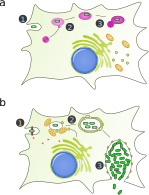
\includegraphics[width=\textwidth]{Parts/Part01/gfx/legionella_life_cycle.pdf}
    \caption[Infection by \textit{Legionella}.]{Infection by \textit{Legionella}: \textbf{a} Non infectious bacteria (green) are phagocytized by amoebae or macrophages (1), the early and late endosomes (pink) acidify the compartment (2), and it finally merges with the lysozome (3) where the bacteria is degraded. \textbf{b} Upon phagocytosis, \textit{Legionella} uses its type IV secretion system to secrete effector proteins (red triangles) into the cytoplasm and evades the endosome route (1). Instead, it stays in a "\textit{Legionella} containing vesicle" (LCV) and recruits mitochondria (orange) and endoplasmic reticulum-derived vescicles (yellow) (2). The bacteria keeps replicating in the LCV until it bursts out and infects other cells.}
	\label{fig:01-01:legionella}
\end{figure}

\subsection{Life cycle}
\textit{L. pneumophila} follows a biphasic life cycle. It can survive in the extracellular environment and thrives in fresh water. It can either spread planktonically as a free living organism using its flagella to reach new hosts, or by associating with biofilms \citep{hilbiLegionellaSppOutdoors2011,steinertLegionellaPneumophilaAquatic2002}. This extracellular phase is called the "transmissive form", as bacteria will search for new host cells but will not replicate \cite{byrneExpressionLegionellaPneumophilaVirulence1998}. In contrast, when entering a host cell, the bacterium enters the "replicative form". In that stage, the  bacterium takes advantage of the abundant resources and nutrient available in the host cell to replicate as much as possible.

Switching between replicative and transmissive phases requires consequent morphogenetic and metabolic changes, mobilizing expression changes in almost half of the known genes \cite{steinertLegionellaPneumophilaAquatic2002}. Low nutrient and high stress conditions cause \textit{L. pneumophila} to enter transmissive phase, activating genes related to motility and virulence, such as its type IV secretion system. When entering the replicative phase, genes related to sugar and gluconate uptake and amino-acid catabolism are upregulated instead. The bacteria become acid resistant and replicate in the \acrshort{LCV} until the nutrient pool is depleted.

Comparison of gene expression profiles between \textit{L. pneumophila} grown \textit{in vitro} in the absence of host, and \textit{in vivo} in the amoeba \textit{A. castellanii} revealed that changes associated with progression from exponential growth to stationary phase are similar to those observed between replicative and transmissive phases \cite{bruggemannVirulenceStrategiesInfecting2006}. In \textit{in vitro} cultures, stationary phase refers to the time when bacteria stop replicating for lack of nutrients. This suggests that the biphasic life cycle of \textit{L. pneumophila} is governed mostly by nutrients present in the environment \cite{olivaLifeCyclePneumophila2018}.

The master regulator underlying this switch is thought to be the carbon storage regulator protein A (CsrA). CsrA is an RNA binding protein with over 400 target transcripts identified, including 40 effector proteins and genes related to virulence and motility. In replicative phase, CsrA binds its target transcripts to repress their translation. When nutrients are running low, \textit{L. pneumophila} produces the alarmone (p)ppGpp, which triggers the expression of noncoding transcripts with strong affinity for CsrA. This prevents CsrA from binding its targets and enables the translation of virulence genes \cite{sahrLegionellaPneumophilaGenome2017}.

\subsection{Host interactions}

While inside the host, \textit{L. pneumophila} consumes products from the host cell for energy production. It relies mainly on serine, threonine and other amino acids but can also scavenge carbohydrates such as gluconate \cite{bruggemannVirulenceStrategiesInfecting2006}. Those nutrients are transferred from the host cytoplasm to the LCV by transporters on the LCV membrane \cite{wielandIntracellularMultiplicationLegionella2005}. The bacterium can increase the availability of nutrients in the host cell using its effector proteins. One example is the AnkB effector which can poly-ubiquitinate host proteins, causing their degradation by the host proteasome, resulting in amino acids which can then be imported into the LCV and consumed \cite{priceMolecularMimicryFBox2009}. Other effectors block host protein translation to increase the pool of free amino acid available for consumption by \textit{L. pneumophila} \cite{deleonPositiveNegativeRegulation2017}.

The host trafficking system is also hijacked, resulting in the recruitment mitochondria and \acrfull{ER} membrane vesicles to the LCV. This is likely achieved by modulating the activity of host GTPases, such as Arf1, Sar1 and Rab1 \cite{isbergLegionellaPneumophilaReplication2009}. Some \textit{Legionella} effectors directly affect the host actin cytoskeleton, which is important in many cellular processes including vesicle trafficking \citep{liuLegionellaEffectorDisrupts2017,francoLegionellaPneumophilaEffector2012}.

\textit{L. pneumophila} also ensures successful infection by promoting host cell survival. The effector SdhA interferes with host cell apoptosis by inhibiting caspases \cite{lagunaLegionellaPneumophilatranslocatedSubstrate2006}. All these interference with the host cell signalling pathways are likely bound to affect its expression program. It was recently found that one of the effectors secreted by \textit{L. pneumophila} directly affects the host epigenetic state. This effector, named RomA, is a histone methyltransferase which can alter the histone methylation state throughout the host genome and affects the expression of a large number of genes \cite{rolandoLegionellaPneumophilaEffector2013}.

There is still much to learn about the interaction between \textit{Legionella} effectors and its host regulation, but that the bacteria is able to modify directly nucleosomes of the host unveiled a new level of intimacy between bacterial endosymbionts and their host, with fascinating perspectives. Besides, epigenetics and gene expression are tightly connected with spatial genome organization in eukaryotes \cite{dixonChromatinDomainsUnit2016,schneiderDynamicsInterplayNuclear2007}, providing a new angle to approach the study of host-pathogen interactions.

\section{\textit{Salmonella enterica}}

Unlike \textit{L. pneumophila}, \textit{S. enterica} infects not only mammals but also birds and reptiles \cite{uzzauHostAdaptedSerotypes2000}. It is also a model for intracellular bacterial infections and a major human pathogen. \textit{Salmonella} is a facultative intracellular parasite which can infect macrophages, dendritic, epithelial and microfold (M) cells. It is usually transmitted by ingestion of contaminated food and colonizes the gastrointestinal tract. \textit{Salmonella} isolates are classified into 2,500 serovars based on their lipopolysaccharides and flagellar antigens. While most serovars, referred to as "non-typhoidal" cause salmonellosis, a self-limiting enteritis, "typhoidal" serovars are human restricted and cause a systemic disease known as typhoid fever \cite{larockSalmonellaeInteractionsHost2015}.

Every year, it is estimated that there are 16.6 million cases of typhoid fever causing 600,000 deaths in the world, and 1.3 billion cases of acute gastroenteritis associated with \textit{Salmonella}, responsible for 3 million deaths \cite{pangTyphoidFeverOther1995}. Most of the current knowledge on \textit{Salmonella} infection biology was built on the non-typhoidal serovar \textit{S. enterica} subsp. \textit{enterica} serovar Typhimurium \cite{larockSalmonellaeInteractionsHost2015}. 

Much like \textit{Legionella}, when \textit{Salmonella} enters the host cell, it is engulfed into a \acrfull{SCV}  and secretes effector proteins into the host cytoplasm. This is done via two independent type 3 secretion systems (T3SS) named SPI1 and SPI2. These two systems are encoded by and named after the \textit{Salmonella pathogenicity island}, which \textit{Salmonella} likely acquired through horizontal gene transfer.

The mechanisms employed by \textit{Salmonella} to infect host cells are similar to \textit{Legionella}. For example, they encode effectors that also activate the host gene Arf1 to promote bacterial uptake and actin polymerization \cite{larockSalmonellaeInteractionsHost2015}. Although no effector of \textit{Salmonella} is known to directly affect the host epigenetic state, a global rewriting of histone modifications and DNA methylation \cite{szteinSalmonellaEntericaSerovar2020,wangChickenCecalDNA2020} is observed in \textit{Salmonella}-infected cells. Furthermore, histone modifications was associated with susceptibility to Salmonella infection in chickens \cite{gouEpigeneticModificationTLRs2012}, further highlighting the importance of investigating chromatin changes during bacterial infection.


 % Chapter 1
% Chapter X

\chapter{Infection through the lense of genomics} % Chapter title

\label{ch:01-02} % For referencing the chapter elsewhere, use \autoref{ch:name} 

%----------------------------------------------------------------------------------------

The toolset to detect and investigate bacterial infection traditionally included biochemical assays and microscopy. The recent technological advances in DNA sequencing have spurred a rapid extension of this toolset with NGS-derived methods. Here we introduce the different ways genomics to provide biological insights into the biology of bacterial pathogens.

\section{Pathogen characterization}

The most fundamental task related to infection in biomedical research is to detect the presence of infectious agents and identify their nature. This allows to test patients presenting suspicious symptoms for the presence of known pathogens, or determine the pathogenicity of a particular strain. 

This is traditionally achieved using molecular biology techniques.

\section{Genomics to probe homeostasis}

When host cells are exposed to or infected by a pathogen, their homeostatic state will be disrupted. This disruption is a combiantion of host-triggered reactions to improve its survival, and alterations caused by the pathogen to colonize the host cell. Untangling these two phenomenon is a complex issue in itself, but investigating what biological functions or pathways are disrupted upon infection can already give good  pointers to important players in the infeciton.

Multiple levels of regulation are affected, from gene expression to epigenetic states, and over the years, a vast arsenal of NGS techniques have been developed to read thse regulatory states. For example, ChIPseq, ...

he transcribed genes, present in the cell in the form of RNA, can also be read using the same DNA sequencing technologies. This allows one to estimate the expression of genes from the amount of RNA present in the cells. This is useful when studying infection, as the expression of each gene can be compared between uninfected and infected cells to detect which biological functions are perturbed.



\section{Capturing chromosome conformation}

The use of genomics to investigate the three-dimensional organisation of the genome started with the invention of \acrfull{3C} \cite{Dekker2002}. This technique allowed to measure the frequency of physical interactions a pair of loci. This is done by crosslinking the genome with formaldehyde, which forms stable bonds between DNA and proteins, and subsequently digesting the genome with a restriction enzyme. The digested genome is then relilgated, and the religation will happen with different neighbouring fragment. Loci which are closer in space will be religated more often with each other in the population of cells. The crosslink is then reverted and qPCR is used to measure the quantity of religated products containing the two loci of interest. 

Since then, many derivative of the \acrshort{3C} technique have been developed. The most significant improvement was brought by Hi-C. This method works similarly to 3C except that next generation sequencing is used instead of qPCR. This allows to quantify the interaction frequency of all versus all loci in the genome instead of using specific primers for a pair of locus. Hi-C also has an additional step where biotinylated bases are added during religation. This allows to pull-down religation products using streptavidin so that only products that underwent the digestion-religation process are sequenced.

Hi-C allows to generate interaction frequency maps of the whole genome wich reflect its 3D structure.

\section{Combining layers of biological informations}

\section{Reproducibility and reliability challenges}
% Impact of the reproducibility crisis
% Software quality
% The importance of standardisation
 % Chapter 2
% Chapter X

\chapter{The importance of genome assembly} % Chapter title

\label{ch:01-03} % For referencing the chapter elsewhere, use \autoref{ch:name} 

%----------------------------------------------------------------------------------------
Most of the genomic techniques presented before require a complete reference genome as downstream analyses will rely on the relative position of different biological elements on the genome sequence to draw biological conclusions. 

A good phylogenetic representation of sequenced genomes is also crucial for comparative analyses. This allows for example to  identify recent \acrshort{HGT} events. Here we describe in more detail the process of genome assembly and its relevance to infection genomics.

\section{From contigs to chromosomes}
% Define terminology, explain advantages of chromosome level assemblies and how to generate them
% Subsections for bionano, linked reads and Hi-C
% Maybe a quick mention of haplotype-resolved assemblies and genome-graphs

Genome assembly consists in reconstructing the linear sequence of the genome from the readings of DNA sequencing technologies. Although the final assembly depends on the quality of these readings, the algorithms used to combine their information are also crucial.

In the early days of genome sequencing, the Sanger method was used to read DNA sequences \cite{sangerDNASequencingChainterminating1977}. Sanger is a low throughput, but highly accurate sequencing method. This technology allowed to unveil the complete genome sequences of viruses \citep{sangerNucleotideSequenceBacteriophage1982,baerDNASequenceExpression1984} and the yeast genome \cite{oliverCompleteDNASequence1992}. A common practice at the time, was to clone a small genomic region of \textasciitilde 10kb into a plasmid, and fragment it \cite{thierryCompleteSequenceKb1990}. The resulting fragments were sequenced and the sequencing readout, in the form of gels, had to be deciphered by scientists, one nucleotide at a time. The cloned region was then assembled manually by searching for overlaps between fragments.

Further technological improvements allowed to automate the sequencing process to tackle the sequencing of larger eukaryotic genomes. Early genome sequencing projects were performed using laborious and costly experimental methods, such as \acrfull{BAC}, which involved cloning long overlapping pieces of DNA of the genome into bacteria. These pieces were then experimentally amplified and sequenced in parallel. Ovelapping ends from each of those sequences had to be aligned to recover the entire chromosome sequence. The first genome sequencing projects were sizable undertakings requiring the collaboration of many research groups throughout the world \citep{collinsNewFiveyearPlan1993,adamsGenomeSequenceDrosophila2000,oliverCompleteDNASequence1992}, but technological advancements progressively reduced the cost and time required. A decisive change was the development of shotgun sequencing \cite{venterSequenceHumanGenome2001}, which involves randomly sequencing regions to cover the entire genome.

With the advent of \acrfull{NGS}, shotgun sequencing became the standard for whole genome sequencing. \acrshort{NGS} has much higher throughput than Sanger sequencing, allowing to sequence megabases of DNA very quickly. However, it can only read short sequences at a time, referred to as \Gls{read}s. Classic overlap-based genome assembly algorithms used in previous sequencing projects could not scale to such large numbers of short reads. This called for the development of more efficient genome assembly algorithms.

The goal of an assembler is to generate a highly contiguous genome sequence from a large number of short reads. Early algorithms computed pairwise alignments between all reads to build an overlap graph (Fig. \ref{fig:01-03:debruijn}a). The genome could then be assembled by finding th e Hamiltonian path of the graph, which passes once through every node. However, finding this approach is computationally expensive and cannot be used with high sequencing throughput \cite{compeauHowApplyBruijn2011}. This lead to the development of de Bruijn-based assembly algorithms, which many most modern still use \citep{simpsonABySSParallelAssembler2009,zerbinoVelvetAlgorithmsNovo2008}. de Bruijn assemblers split reads into short \Gls{k-mer}s which they use to generate a de Bruijn graph. In these graphs, k-mer sequences represent edges, and the overlap between adjacent k-mers within reads are the nodes (Fig. \ref{fig:01-03:debruijn}b). To assemble a genome, assemblers need to find the Eulerian path, which passes through every edge once. However this is often not possible because of repeated sequences in the genome, sequencing errors and haplotypes \cite{simpsonTheoryPracticeGenome2015}. Whenever a repeated sequence is longer than the read itself, the graph can not be solved and heuristics have to be used. Rather than a single fully resolved genome, the resulting assemblies usually have a relatively high number of independent pieces called \Gls{contig}s.

\begin{figure}
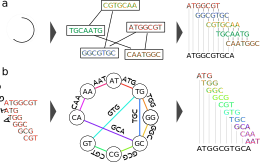
\includegraphics[width=\textwidth]{Parts/Part01/gfx/debruijn.pdf}
\caption[Graphs in genome assembly.]{Graphs in genome assembly: A small circular genome is sequenced and the resulting reads are shown in color \textbf{a}: Early assembling techniques computed all pairwise alignments between reads to represent them as nodes in an overlap graph and their overlaps as edges. The genome sequence can be retrieved by finding a path going through each read exactly once. \textbf{b}: Modern assemblers first split reads into their constituent k-mers and represent the k-mers as edges in a de Bruijn graph where nodes are the k-1 overlap between two k-mers located in the same read. The path going through each edge once is computed to solve the graph. K-mers are extracted from the edges visited to retrieve the genome sequence. Adapted from \cite{compeauHowApplyBruijn2011}}
\label{fig:01-03:debruijn}
\end{figure}

Third generation sequencing partially alleviates this issue by generating long albeit less accurate reads. Read lengths up to hundreds of thousands of basepairs can be generated, which allows to span most repeated regions. Recently, these technologies were used to generate telomere-to-telomere assemblies of several human chromosomes \citep{migaTelomeretotelomereAssemblyComplete2020,logsdonStructureFunctionEvolution2021}. Third generation sequencing techniques still suffer from their lower base calling accuracy resulting in assemblies with high point error rates (>10\%) and indels \cite{weiratherComprehensiveComparisonPacific2017,jainNanoporeSequencingAssembly2018}. To remove these errors, some methods have been developed to correct long reads before assembly, either by correcting long reads among themselves \cite{morisseScalableLongRead2021}, or using a separate set of short accurate reads to erase sequencing errors in long reads \cite{wangFMLRCHybridLong2018}. Most long reads correction tools are also unable to differentiate between SNPs and sequencing errors, which result in the loss of haplotype information and prevents the generation of haplotype-resolved assemblies. Some long read correction methods have recently been developed to preserve haplotypes information \cite{holleyRatatoskHybridError2021}. One major drawback of read correction methods is their high computational cost, as they require to align high number of reads to each others. An alternative strategy is to use the uncorrected reads to assemble the genome and perform errror correction directly on the assembly, a process known as \Gls{polishing}. Traditional short read polishers work by aligning short reads to the assembly and replacing each position of the assembly by the consensus of short reads \cite{vaserFastAccurateNovo2017}. Additionally, they can correct larger scale misassemblies such as indels by using the pair-end information and alignment discrepancies \cite{walkerPilonIntegratedTool2014}. Some polishers have obtained better polishing accuracy by combining the information in short and long reads \cite{kunduHyPoSuperFast2019}.

More recently the emergence of specialized technologies aimed at scaffolding have allowed to generate even more continuous and correct genomes at reduced costs. One example is the recent rebirth of optical mapping to introduce fluorescent probes into chromosomes at specific sites \cite{lamGenomeMappingNanochannel2012}. The order of these probes and their relative distance form barcodes which can then be used to scaffold genome assemblies, reorder and merge contigs. This is often combined with Hi-C to generate highly continuous assemblies even in the presence of repeated sequences.

A growing number of genome assemblies combine several of these different technologies to bring the number of scaffolds as close as possible to the real number of chromosomes (Fig. \ref{fig:01-03:assembly}).

\begin{figure}[htb]
    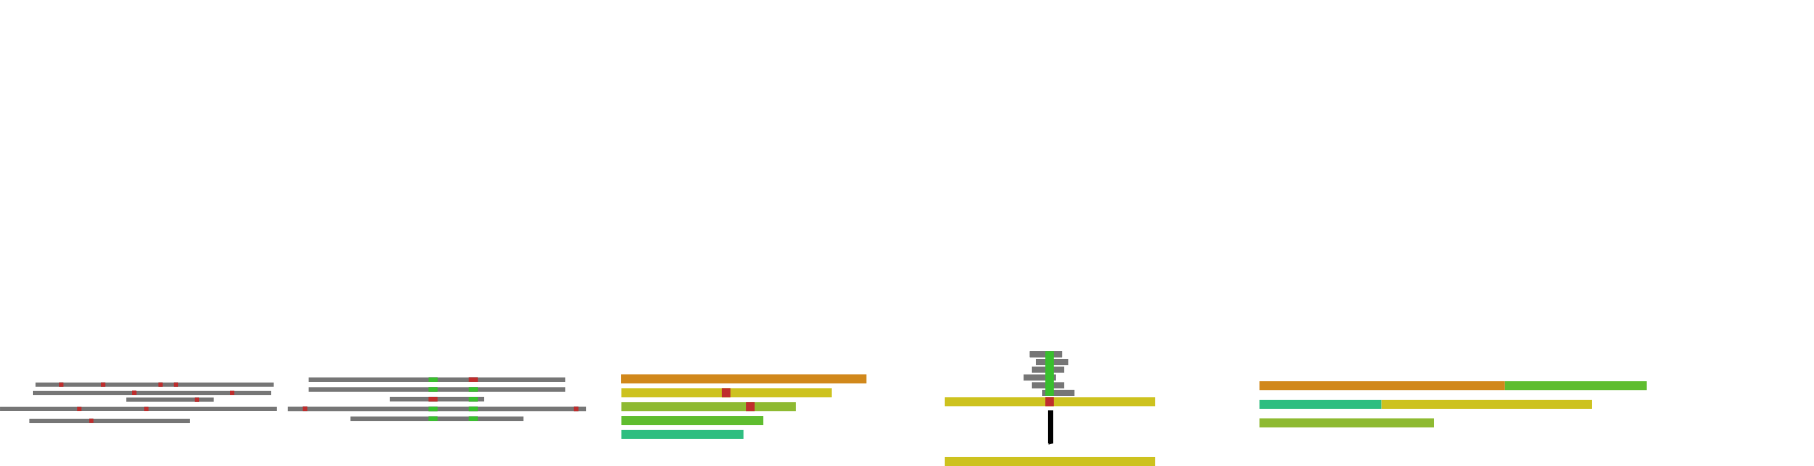
\includegraphics[width=\textwidth]{Parts/Part01/gfx/assembly_pipeline.pdf}
    \caption[Example of a third generation sequencing assembly pipeline.]{Example of a typical assembly pipeline using third generation sequencing. The error prone long reads are first corrected by pairwise comparisons. The corrected reads are assembled into contigs using their overlaps. The remaining sequencing errors in the assembly are removed by polishing with accurate short reads. Other sources of information can then be used to combine contigs into scaffolds.}
    \label{fig:01-03:assembly}
\end{figure}

\section{Phylogenetic representation}
% HGT detection requires a reference group

A common way to analyze the genome of new microorganisms is to compare it to other species. To achieve this, one needs to have other closely related genomes available. A common case where dense species genome representation is required is when attempting to detect \acrshort{HGT}.

\acrshort{HGT} detection methods often rely on discordance between gene trees and species trees. A horizontally transferred gene between two distant species would show strong sequence similarity \cite{ravenhallInferringHorizontalGene2015}. For this reason, detection of recent events requires genomes of closely related organisms as a comparison point.

\begin{figure}[htb]
    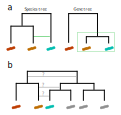
\includegraphics[width=\textwidth]{Parts/Part01/gfx/phylo_hgt.pdf}
    \caption[Phylogenetic representation of an HGT event.]{Phylogenetic representation of an HGT event. \textbf{a:} An HGT event between two species (shown with a green arrow) can be detected through discrepencies between the species (left) and gene (right) trees. \textbf{b:} In cases where genomes of closely related species are unavailable (greyed out organisms), the origin of the horizontal transfer cannot be accurately inferred (possible events shown with grey arrows).}
    \label{fig:01-03:phylo-hgt}
\end{figure}

Another frequent analysis when comparing a group of strains or species of microorganisms is to define the common set of genes they share, known as pangenome. This also allows the identification of genes specific to a particular genome, known as accessory genome. Such sets can be helpful to determine metabolic reactions associated with species or niches, however they heavily depend on the proportion of available species in the group.

Lately, several large consortia \citep{genome10kcommunityofscientistsGenome10KProposal2009,poelchauI5kWorkspaceNAL2015,DarwinTreeLife} undertook the daunting task of sequencing thousands of organisms throughout the tree of life. For the aforementioned reasons, these large collaborations are likely to greatly improve the power of comparative genomic analyses results in the future.

\section{The transition to genome graphs}

Until recently, all reference genomes were exclusively stored as linear (or circular) sequences of DNA. This linear sequence is often obtained from a mix of multiple individuals, or alleles within an individual. It is effectively a semi-arbitrary combination of multiple haplotypes collapsed into an artificial consensus sequence. A more accurate alternative is to produce a reference sequence graph instead \cite{churchExtendingReferenceAssembly2015}. Given a collection of haplotypes, individuals, or strains of a species, one can generate a graph where identical regions are collapsed, while sample-specific variants form bubbles retaining the genetic variability. As this approach is relatively recent, few algorithms have been developed to operate on sequence graphs, making their applications very limited.

The shift to genome graphs is promising for the analysis of bacterial samples, where alignment can be performed on multiple strain references at the same time. Doing this with a collection of linear genome incurs mapping bias due to ambiguous alignments between redundant regions between references \cite{liDesignConstructionReference2020}. Similarly, genome graphs also allow systematic alignment to different alleles in polyploid organisms, solving the issue of allele-specific mapping bias in linear references \cite{vandegeijnWASPAllelespecificSoftware2015}.  % Chapter 3
%% Chapter X

\chapter{Thesis objectives} % Chapter title

\label{ch:01-04} % For referencing the chapter elsewhere, use \autoref{ch:name} 

Throughout this first part, we have laid out the scope of host-pathogen interactions and summarized the current state of genomics in relation to regulation and 3D genomes. Although genomics is a fast changing field, there is a need for computational tools to extract meaningful biological information from the wealth of data.

Throughout the next part, we will introduce our contributions to the field and main results. In the first chapter, we explain our methodological developments related to chromosome conformation capture technologies. In the second chapter, we will present our chromosome scale genome assembly of \textit{A. castellanii}. We then use this resource for our main findings on the genomic changes happening during infection by \textit{L. pneumophila}. Chapter 3 will focus on murine bone macrophages infection by \textit{S. enterica} and the genomic alterations it entails. Finally, in chapter 4, we will discuss additional results related to the implications of viral integrations linked to hepatocellular carcinoma in the human genome. We will end with part 3 where we discuss various aspects of genomics in infection biology, including prospects and limitations.

In this work, we develop accessible and performant methods to extract information from 3C technologies and use them to identify changes happening during infections in various organisms. We then use external data such as gene expression to assess the genes involved in those alterations and discuss how they could be associated with the infection process.
%----------------------------------------------------------------------------------------

 % Chapter 4 
\cleardoublepage % Empty page before the start of the next part
%
%%------------------------------------------------
%
\ctpartquote{\cleanchapterquote{Unfortunately, no one can be told what The Matrix is. You'll have to see it for yourself.}{Morpheus}{The Matrix}}

\ctparttext{In this second part, we present new results produced in the frame of this work. We start by describing tools and algorithms developed to address the questions at hand. In later parts, we dive into the biological results and discuss their significance.
}

\part{Results} % Second part of the thesis


% Chapter X

\chapter{Extracting information from contact maps} % Chapter title

\label{ch:02-01} % For referencing the chapter elsewhere, use \autoref{ch:name} 

%----------------------------------------------------------------------------------------

Most genomics methods generate a large amount of information, most of which is not directly relevant for the problem at hand. One of the main challenges emanating from genomics data is to distill this information and extract only the relevant signal.

In the case of Hi-C and other 3D genomics techniques, the resulting signal is a list of contacts between pairs of genomic regions. These contacts reflect the average genome structure from a population of cells and are subject to various biases.

The spatial features and changes of interest are diluted in the population and can be obfuscated by noise. Detecting these changes requires a set of bias correction and signal detection methods which are still in their early developments.

In this section we review the recent methodlogical developments that allow to correct the Hi-C signal and present new methods to extract biological features from these datasets. These developments proved necessary to tackle the questions raised in further chapters.

\section{Streamlined and reproducible Hi-C processing}
% Existing methods: painful to install, non tested (risky), non reproducible
% hicstuff, hicreppy

The pre-processing of Hi-C data itself, to convert \acrfull{NGS} reads into chromosomal contact matrices involves several steps that will impact the resulting signal.

The sequencing reads themselves can be the result from religation of two distinct loci. These chimeric reads cannot be aligned reliably with generic methods and need to be cut for proper alignment. Chimeric reads become more problematic when increasing the read size relative to restriction fragment length.

Not all read pairs generated by Hi-C experiments represent valid spatial interactions. Some restriction fragments are sequenced without religation and other fragments religate on themselves. The various interaction types can be separated based on the strand of origin of their individual reads. In theory, and in practice at long ranges, one would expect religations to be strand agnostic and to have an equal represenation of all four possible combinations (++, --, +-, -+). In reality, this is never the case at short range contacts, due to the enrichment of self-religation (-+) and dangling ends (or undigested fragments, +-).

These biases must be accounted when processing Hi-C data. This can be achieved by identifying and filtering out faulty interactions based on their strands.

This preprocessing is often performed using custom scripts and prone to errors, butgs and lack of informations about parameters. In an effort to improve reproducibility and accessibility of Hi-C analysis, we developed hicstuff, an open source Hi-C pipeline that incorporate all the aforementioned steps, along with several downstream processing utilities.

Hicstuff is meant to be easily accessible, even to non-expert users. It has a comprehensive online documentation and tutorials and the program and its dependencies are installed with a single command. The code is written in python, and is covered by unit tests to reduce the likelihood of bugs. Hicstuff runs well with default parameters, but has many options to fit most common use cases. It works regardless of genome size organism.

The pipeline also provides reproducibility through an automatic logging of every intermediate result in the pipeline as well as the input parameters used.

The project has already fostered a community of users which are offering their contributions, suggest features or report issues they encounter.

\section{Feature detection with Chromosight}

The downstream analysis of chromosome contact maps often involves looking for signals reflecting biologically relevant spatial interactions. Several specialized approaches for pattern detection have been proposed in the past. Each of these methods use a set of specific rules to detect one particular type of pattern. For example, HICCUPS \cite{rao3DMapHuman2014} detects chromatin loops by scanning each pixel of the contact map for contact enrichment compared to surrounding pixels.

These specialized methods present several drawbacks, including strong dependence on parameters and poor generalization to non-model species. These shortcomings motivated us to work on a more generalized pattern detection method that uses template matching to identify arbitrary patterns in chromosome contact maps.

\section{Change detection across biological conditions}

Change detection is a common issue in the field of signal processing and remote sensing. Given two or more input signals such as images, we want to find portions that differ between the two inputs. This principle can also be applied to Hi-C contacts, where we can detect regions of contact maps that differ between biological conditions.

Change detection in Hi-C contact maps is required whenever we want to identify genomic regions whose spatial organization is altered between two conditions.

Many approaches can be taken to detect these changes. Some of them, such as diffhic, formulate the problem similarly to a differential expression RNAseq analysis using contact counts instead of read counts. This approach has the benefit of being statistically sound and straightforward, but it only finds contact increase. Local increase in contacts can represent a specific spatial interactions, but also differential accessibility or insulation. which could be caused by a number of different phenomenon.

We developed pareidolia, a software package for change detection with an apriori on the type of signal to detect. The method is "supervised" in the sense that it requires a kernel representing the feature of interest. Pareidolia relies on Chromosight's backend to convert the contact map of each condition into a map of correlation coefficients representing similarity with the feature of interest. Change detection is then performed on these coefficients. As a consequence, rather than looking for contacts increase, pareidolia looks for changes in feature intensity, such as border sharpness or looping intensity.

\subsection{Pareidolia algorithm}

Pareidolia works by comparing one or several samples issued from two or more conditions such as treatments or timepoints.

Assuming two conditions $t={t_0, t_1}$, where multiple samples (replicates) $(r_1, r_2, ..., r_R)$ can share the same condition. The contact matrix from each sample $H_{r, t}$ is first convoluted with a kernel $K$ representing the pattern of interest. In the resulting matrix $M$, each value $M_{r, t}[i, j]$ is a Pearson correlation coefficient with the kernel. $M$ is computed as described in equation...


Change detection can then be performed on the correlation maps using two different methods.

The first method is inspired by median filtering-based background formation. We start by generating a background matrix for each condition (timepoint), whose values are defined as the median of all replicates in that condition: 

\begin{equation}
    B_t[i, j] = median(M_{1, t}, M_{2, t}, ..., M_{R, t})
\end{equation}

We then compute the matrix of absolute variations $V$ between each replicate and their condition's median background. The resulting distribution is used to define a percentile threshold of technical variation.

\begin{align}
    V_t &= M_{r, t} - B_t \\
    T &= Q_{V_{t0},V_{t1}}(0.95)
\end{align}

The alternative method is to compute a test statistic and associated p-value for every pixel [i,j], and then select contiguous regions of strong changes. % Chapter 1
% Chapter X

\chapter{Infection of \textit{Acanthamoeba castellanii} by \textit{Legionella pneumophila}} % Chapter title

\label{ch:02-02} % For referencing the chapter elsewhere, use \autoref{ch:name} 

%----------------------------------------------------------------------------------------

\section{Genome assembly}

\section{Strains comparison}

\section{Changes during infection}

\blindtext % Chapter 2
\textsc{}% Chapter X

\chapter{Infection of murine macrophages by \textit{Salmonella}} % Chapter title

\label{ch:02-03} % For referencing the chapter elsewhere, use \autoref{ch:name} 

%----------------------------------------------------------------------------------------

In this chapter, we investigate whether, and how \textit{Salmonella enterica} infection can affect the chromatin regulation of its eukaryotic host. Much like \textit{Legionella}, \textit{Salmonella} manipulates its host cell's defense and signalling to promote its own survival in their cytoplasm \cite{larockSalmonellaeInteractionsHost2015}. Using a mouse \acrfull{BMM} model, we measure changes in chromatin architecture, accessibility and gene expression in different infection conditions and timepoint to explore the potential epigenetic deregulations happening during this process.

While in previous chapter, we investigated changes during infection in a unicellular host, here we are using a mammalian host. Mammal genomes have a complex organizaton, they are much larger and segmented into active and inactive compartments. They contain regulatory elements organized into chromatin domains and exhibiting cell type specificity \cite{schmittCompendiumChromatinContact2016}.

Here we focus on bone marrow-derived macrophages. These cells originate from hematopoietic stem cells and go through a complex differentiation process (Fig. \ref{fig:02-03:macrophage}a). After differentiation, they have a strong plasticity and can be activated by cues in their environment to become "polarized" into one of two main activation states (Fig. \ref{fig:02-03:macrophage}b). M1 macrophages secrete high amounts of cytokines and promote inflammation, while M2 macrophages suppress immune response and focus on tissue repair \cite{ahmedM1M2Macrophages2020}. M1 Macrophages are key cells during response to bacterial infection, as they will phagocytose bacterial cells and initiate adaptive immunity by activating T cells through antigen presentation via the Major Histocompatibility Complex II (MHC-II). Additionally, they will produce chemokines to promote inflammation and recruit other immune cells, and secrete anti-microbial molecules to destroy infectious cells. However, in case of prolonged infection, this strong immune reaction can actually be detrimental to the host by causing organ damage, or even lethal shock \cite{magesGenomewideAnalysisLPS2008}. This overstimulation is avoided by a process known as endotoxin- or LPS-tolerance. This state of reduced immune response is triggered by continuous exposure to lipopolysaccharides exposed on the bacterial cell surface and skews the macrophage population towards M2 polarization \cite{portaToleranceM2Alternative2009}. However, LPS-tolerance must also be tightly balanced, as suppressed immunity can lead to secondary infection or even sepsis. Such regulation is known to involve a combination of signalling and gene-specific chromatin changes through histone modifications \cite{aungLPSRegulatesProinflammatory2006}.

 Throughout the next sections, we will investigate chromosome conformation changes in macrophages following infection by \textit{Salmonella}. As we will focus on changes happening during late infection, LPS-tolerance is especially relevant to the understanding of this chapter.

\begin{figure}[htb]
    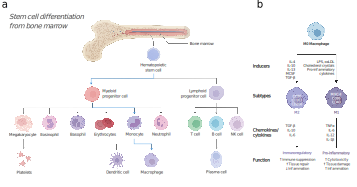
\includegraphics[width=\textwidth]{Parts/Part02/gfx/macrophage_differentiation.png}
    \caption[Macrophage differentiation.]{Macrophage differentiation from hematopoietic stem cells. \textbf{a:} Cellular differentiation pathway leading from bone marrow stem cells to macrophages \textbf{b:} Macrophage polarization from M0 to M1 (pro-inflammatory) or M2 (anti-inflammatory) macrophages. For either forms, molecules associated with induction of polarization, surface exposure and secretion are listed, as well as its functions. Adapted from "Stem cell differentiation from bone marrow" and "Macrophage subtypes in atherosclerosis", by BioRender.com (2020). Retrieved from https://app.biorender.com/biorender-templates}
    \label{fig:02-03:macrophage}
\end{figure}


\includepdf[pages=-,addtotoc={
     1,section,1,Alteration of chromatin structure in macrophages during infection by \textit{Salmonella},p1,
     1,subsection,2,Introduction,sec:02-03:se-int,
     2,subsection,2,Results,sec:02-03:se-res,
     4,subsection,2,Discussion,sec:02-03:se-dis,
     7,subsection,2,Methods,sec:02-03:se-met,
     12,subsection,2,Supplementary figures,sec:02-03:se-sup}]
     {Publications/mouse_salmonella_manuscript.pdf}     % Chapter 3
% % Chapter X

\chapter{Viral insertions in the human genome} % Chapter title

Viruses represent another type of host pathogen interactions. Some of those viruses, including the hepatitis B virus (HBV), have the ability to insert their genetic material into the genome of their host. Depending on the genomic landscape around those insertions, it can have various effects on the host cells.

It is known that hepatocellular carcinoma (HCC), a type of liver cancer, are frequently associated with HBV insertions.

Here we investigate the location of those viral insertions in multiple HCC cell lines, the epigenetic marks present at those regions and how they affect the local 3D structure.

\label{ch:02-04} % For referencing the chapter elsewhere, use \autoref{ch:name} 

%-----------------------------------------------------------------------------------

\section{Genome structure of HBV-infected cancer cell lines}

\section{Detection of viral insertions}

\section{Epigenetic states at inserted regions}

\blindtext % Chapter 4
\cleardoublepage % Empty page before the start of the next part
%
%%------------------------------------------------
%
\ctpartquote

\ctparttext{In this last part, we discuss the findings from this work and place them in the context of the field in its current state. We also discuss the limitations of our approaches and how to improve on it. Finally we briefly reflect upon future developments and perspectives for chromosome conformation analyses in infection biology.}

\part{Discussion and conclusion} % Second part of the thesis
% Chapter X

\chapter{Limitations of genomics in infection biology} % Chapter title

\label{ch:03-01} % For referencing the chapter elsewhere, use \autoref{ch:name} 

%----------------------------------------------------------------------------------------


\section{Correlation is not causality}


\section{Reproducibility and reliability challenges}
% Impact of the reproducibility crisis
Results from genomics analyses are especially sensitive to the parameters and methods used. This makes reproducibility in bioinformatics of utmost importance. Just like RNAseq, Hi-C has important technical variability which needs to be accounted for using multiple replicates.

It was proposed that RNAseq experiments for differential expression analysis should comprise at least 6 replicates and ideally 12 \cite{schurchHowManyBiological2016}. While this is probably true for most omics experiments, this entails a high cost which is often the limiting factor when designing experiments in genomics.

The core issue with low replicate numbers is the impossibility to distinguish between technical variability due to the assay and biological variability of interest. As a consequence, when fewer replicates are used, lower effect size (fold changes in the case of gene expression) become undetectable. This is especially problematic when studying gene regulation, where small changes in expression can be important.

% Mention beyond p-values ?

% Software quality
Unlike RNAseq, where the standard for analyses is well established and most softwares are able to account for replicates and experimental design, most softwares available for Hi-C analysis cannot use replicate information. This limits the power of analysis to detect only very strong changes. The lack of standard also causes a general fragmentation of bioinformatic tools, with many redundant tools of variable quality. One recurrent issue is the absence or low quality of unit tests and documentation, which are unfortunately still not regarded as standard in the computational biology community. Unit tests could be viewed as an equivalent to control experiments in molecular biology, as they validate each logic piece of the software using inputs with known truths. Software lacking these controls is more likely to have undetected bugs that could impact results and lead to false conclusion.
% The importance of standardisation
Another issue with newer techniques like Hi-C is the lack of standardisation for file formats and practices. This can result in incompatibilities between programs and introduce errors during conversions that alter the data.

Some general practices can of course be adopted to address these issues, such as writing comprehensive documentation, solid tests and maintain software, but as it stands, there is no incentive to do so in academia. Ultimately, these directives need to be enforced globally in the peer review process by journals, so that tools need to meet quality standards to reach publication.

Although this will increase the effort and time required to develop methods, this also means the resulting tools will be more reliable, easier to use and more widely adopted. Fortunately, recent years have seen an increasing adoption of good practices in bioinformatic software and the cool format is now supported by the majority of Hi-C analysis tools. This could mean that the quality of academic software for bioinformatics will undergo major improvements in the forseeable future.  % Chapter 1
% Chapter X

\chapter{Perspectives of genomics for infection biology} % Chapter title

\label{ch:03-02} % For referencing the chapter elsewhere, use \autoref{ch:name} 

%----------------------------------------------------------------------------------------

\section{The 3D genome and the advent of deep learning}
% Deepnog (annotation)
% DeepHiC, SRHic, ...(resolution)
% akita & deepc
In some cases, it may be attractive to produce a model of the 3D genome, be it to predict its structure, or how it reacts to specific changes. However, in many organisms, the rules governing genome organization are intricate and it would be unwieldly to model them explicitely. Deep learning provides an attractive framework to produce such a model without knowing all the rules involved. There are already successful applications of deep learning in biology for various different tasks such as gene annotation \cite{stiehlerHelixerCrossspeciesGene2020}, variant calling \cite{poplinUniversalSNPSmallindel2018}, classification of coding RNA \cite{hillDeepRecurrentNeural2018} and perhaps most importantly, protein structure prediction \cite{jumperHighlyAccurateProtein2021}.

%cite akita and deep3C
Generally, applications of deep learning in the 3D genome field have been limited to denoising or improving the resolution of Hi-C matrices. Recently however, there have been successful attempts at predicting the structure of mammalian genomes from the DNA sequence, and even predict conformational changes induced by mutations. In the future, these approaches could be helpful to select mutants, or regions to focus on, and one could imagine it being used to model the consequences of infection on the host.

Unfortunately, several limitations that must be overcome before deep learning methods can become useful to understand the relationship between biological processes and genome structure. First, it requires enormous amounts of training data, which in the case of Hi-C is very expensive to generate. Then, in the event that such a model could effectively predict conformational changes, in most cases this is insufficient. The end goal is usually to understand the rules and factors that connect the biological process (e.g. infection) to structural changes. In deep learning models these rules are obscured, taking the form of large weight matrices, and extracting them would require consequent advances in model interpretability \cite{talukderInterpretationDeepLearning2021}.
 % Chapter 2
% Chapter X

\chapter{Future perspective} % Chapter title

\label{ch:03-03} % For referencing the chapter elsewhere, use \autoref{ch:name} 

As 3C protocols improve and the cost of sequencing decreases, it will be possible to probe finer details of spatial regulation during bacterial infection. While current projects are mostly limited to analyzing major changes, higher sequencing depth and increasing numbers of replicates should allow for more contrast and with it, the detection of more subtle changes in spatial interactions.

% Single cell (spatial heterogeneity)
Another exciting point is the advent of single-cell omics methods. This is especially interesting for infection genomics, where bulk Hi-C signal contains a mixture of cells at different infection stage and cell cycle phase. These single-cell methodologies may allow to further refine the analysis and deconvolute different effects obscuring the signal of interest.

This work is still among the first of its kind and we expect to see major developments in the use of 3D genomics to understand dysregulation in infection. There is still much to be learnt in the interplay of the various layers of regulation, and spatial organization will likely become an integrative part of many projects aiming to understand it.

%----------------------------------------------------------------------------------------
 % Chapter 3
%% Chapter X

\chapter{Thesis objectives} % Chapter title

\label{ch:01-04} % For referencing the chapter elsewhere, use \autoref{ch:name} 

Throughout this first part, we have laid out the scope of host-pathogen interactions and summarized the current state of genomics in relation to regulation and 3D genomes. Although genomics is a fast changing field, there is a need for computational tools to extract meaningful biological information from the wealth of data.

Throughout the next part, we will introduce our contributions to the field and main results. In the first chapter, we explain our methodological developments related to chromosome conformation capture technologies. In the second chapter, we will present our chromosome scale genome assembly of \textit{A. castellanii}. We then use this resource for our main findings on the genomic changes happening during infection by \textit{L. pneumophila}. Chapter 3 will focus on murine bone macrophages infection by \textit{S. enterica} and the genomic alterations it entails. Finally, in chapter 4, we will discuss additional results related to the implications of viral integrations linked to hepatocellular carcinoma in the human genome. We will end with part 3 where we discuss various aspects of genomics in infection biology, including prospects and limitations.

In this work, we develop accessible and performant methods to extract information from 3C technologies and use them to identify changes happening during infections in various organisms. We then use external data such as gene expression to assess the genes involved in those alterations and discuss how they could be associated with the infection process.
%----------------------------------------------------------------------------------------

 % Chapter 4     

\cleardoublepage % Empty page before the start of the next part
%
%%------------------------------------------------
%
%\ctpartquote{quote}
\ctparttext{\blindtext} % Text on the Part 2 page describing the content in Part 2

\part{PART} % Second part of the thesis
% Chapter X

\chapter{Limitations of genomics in infection biology} % Chapter title

\label{ch:03-01} % For referencing the chapter elsewhere, use \autoref{ch:name} 

%----------------------------------------------------------------------------------------


\section{Correlation is not causality}


\section{Reproducibility and reliability challenges}
% Impact of the reproducibility crisis
Results from genomics analyses are especially sensitive to the parameters and methods used. This makes reproducibility in bioinformatics of utmost importance. Just like RNAseq, Hi-C has important technical variability which needs to be accounted for using multiple replicates.

It was proposed that RNAseq experiments for differential expression analysis should comprise at least 6 replicates and ideally 12 \cite{schurchHowManyBiological2016}. While this is probably true for most omics experiments, this entails a high cost which is often the limiting factor when designing experiments in genomics.

The core issue with low replicate numbers is the impossibility to distinguish between technical variability due to the assay and biological variability of interest. As a consequence, when fewer replicates are used, lower effect size (fold changes in the case of gene expression) become undetectable. This is especially problematic when studying gene regulation, where small changes in expression can be important.

% Mention beyond p-values ?

% Software quality
Unlike RNAseq, where the standard for analyses is well established and most softwares are able to account for replicates and experimental design, most softwares available for Hi-C analysis cannot use replicate information. This limits the power of analysis to detect only very strong changes. The lack of standard also causes a general fragmentation of bioinformatic tools, with many redundant tools of variable quality. One recurrent issue is the absence or low quality of unit tests and documentation, which are unfortunately still not regarded as standard in the computational biology community. Unit tests could be viewed as an equivalent to control experiments in molecular biology, as they validate each logic piece of the software using inputs with known truths. Software lacking these controls is more likely to have undetected bugs that could impact results and lead to false conclusion.
% The importance of standardisation
Another issue with newer techniques like Hi-C is the lack of standardisation for file formats and practices. This can result in incompatibilities between programs and introduce errors during conversions that alter the data.

Some general practices can of course be adopted to address these issues, such as writing comprehensive documentation, solid tests and maintain software, but as it stands, there is no incentive to do so in academia. Ultimately, these directives need to be enforced globally in the peer review process by journals, so that tools need to meet quality standards to reach publication.

Although this will increase the effort and time required to develop methods, this also means the resulting tools will be more reliable, easier to use and more widely adopted. Fortunately, recent years have seen an increasing adoption of good practices in bioinformatic software and the cool format is now supported by the majority of Hi-C analysis tools. This could mean that the quality of academic software for bioinformatics will undergo major improvements in the forseeable future.  % Chapter 1
% Chapter X

\chapter{CHAP} % Chapter title

\label{ch:04-02} % For referencing the chapter elsewhere, use \autoref{ch:name} 

%----------------------------------------------------------------------------------------

\section{SEC}

\blindtext % Chapter 2
% Chapter X

\chapter{The importance of genome assembly} % Chapter title

\label{ch:01-03} % For referencing the chapter elsewhere, use \autoref{ch:name} 

%----------------------------------------------------------------------------------------
Most of the genomic techniques presented before require a complete reference genome as downstream analyses will rely on the relative position of different biological elements on the genome sequence to draw biological conclusions. 

A good phylogenetic representation of sequenced genomes is also crucial for comparative analyses. This allows for example to  identify recent \acrshort{HGT} events. Here we describe in more detail the process of genome assembly and its relevance to infection genomics.

\section{From contigs to chromosomes}
% Define terminology, explain advantages of chromosome level assemblies and how to generate them
% Subsections for bionano, linked reads and Hi-C
% Maybe a quick mention of haplotype-resolved assemblies and genome-graphs

Genome assembly consists in reconstructing the linear sequence of the genome from the readings of DNA sequencing technologies. Although the final assembly depends on the quality of these readings, the algorithms used to combine their information are also crucial.

In the early days of genome sequencing, the Sanger method was used to read DNA sequences \cite{sangerDNASequencingChainterminating1977}. Sanger is a low throughput, but highly accurate sequencing method. This technology allowed to unveil the complete genome sequences of viruses \citep{sangerNucleotideSequenceBacteriophage1982,baerDNASequenceExpression1984} and the yeast genome \cite{oliverCompleteDNASequence1992}. A common practice at the time, was to clone a small genomic region of \textasciitilde 10kb into a plasmid, and fragment it \cite{thierryCompleteSequenceKb1990}. The resulting fragments were sequenced and the sequencing readout, in the form of gels, had to be deciphered by scientists, one nucleotide at a time. The cloned region was then assembled manually by searching for overlaps between fragments.

Further technological improvements allowed to automate the sequencing process to tackle the sequencing of larger eukaryotic genomes. Early genome sequencing projects were performed using laborious and costly experimental methods, such as \acrfull{BAC}, which involved cloning long overlapping pieces of DNA of the genome into bacteria. These pieces were then experimentally amplified and sequenced in parallel. Ovelapping ends from each of those sequences had to be aligned to recover the entire chromosome sequence. The first genome sequencing projects were sizable undertakings requiring the collaboration of many research groups throughout the world \citep{collinsNewFiveyearPlan1993,adamsGenomeSequenceDrosophila2000,oliverCompleteDNASequence1992}, but technological advancements progressively reduced the cost and time required. A decisive change was the development of shotgun sequencing \cite{venterSequenceHumanGenome2001}, which involves randomly sequencing regions to cover the entire genome.

With the advent of \acrfull{NGS}, shotgun sequencing became the standard for whole genome sequencing. \acrshort{NGS} has much higher throughput than Sanger sequencing, allowing to sequence megabases of DNA very quickly. However, it can only read short sequences at a time, referred to as \Gls{read}s. Classic overlap-based genome assembly algorithms used in previous sequencing projects could not scale to such large numbers of short reads. This called for the development of more efficient genome assembly algorithms.

The goal of an assembler is to generate a highly contiguous genome sequence from a large number of short reads. Early algorithms computed pairwise alignments between all reads to build an overlap graph (Fig. \ref{fig:01-03:debruijn}a). The genome could then be assembled by finding th e Hamiltonian path of the graph, which passes once through every node. However, finding this approach is computationally expensive and cannot be used with high sequencing throughput \cite{compeauHowApplyBruijn2011}. This lead to the development of de Bruijn-based assembly algorithms, which many most modern still use \citep{simpsonABySSParallelAssembler2009,zerbinoVelvetAlgorithmsNovo2008}. de Bruijn assemblers split reads into short \Gls{k-mer}s which they use to generate a de Bruijn graph. In these graphs, k-mer sequences represent edges, and the overlap between adjacent k-mers within reads are the nodes (Fig. \ref{fig:01-03:debruijn}b). To assemble a genome, assemblers need to find the Eulerian path, which passes through every edge once. However this is often not possible because of repeated sequences in the genome, sequencing errors and haplotypes \cite{simpsonTheoryPracticeGenome2015}. Whenever a repeated sequence is longer than the read itself, the graph can not be solved and heuristics have to be used. Rather than a single fully resolved genome, the resulting assemblies usually have a relatively high number of independent pieces called \Gls{contig}s.

\begin{figure}
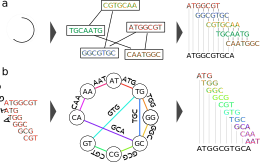
\includegraphics[width=\textwidth]{Parts/Part01/gfx/debruijn.pdf}
\caption[Graphs in genome assembly.]{Graphs in genome assembly: A small circular genome is sequenced and the resulting reads are shown in color \textbf{a}: Early assembling techniques computed all pairwise alignments between reads to represent them as nodes in an overlap graph and their overlaps as edges. The genome sequence can be retrieved by finding a path going through each read exactly once. \textbf{b}: Modern assemblers first split reads into their constituent k-mers and represent the k-mers as edges in a de Bruijn graph where nodes are the k-1 overlap between two k-mers located in the same read. The path going through each edge once is computed to solve the graph. K-mers are extracted from the edges visited to retrieve the genome sequence. Adapted from \cite{compeauHowApplyBruijn2011}}
\label{fig:01-03:debruijn}
\end{figure}

Third generation sequencing partially alleviates this issue by generating long albeit less accurate reads. Read lengths up to hundreds of thousands of basepairs can be generated, which allows to span most repeated regions. Recently, these technologies were used to generate telomere-to-telomere assemblies of several human chromosomes \citep{migaTelomeretotelomereAssemblyComplete2020,logsdonStructureFunctionEvolution2021}. Third generation sequencing techniques still suffer from their lower base calling accuracy resulting in assemblies with high point error rates (>10\%) and indels \cite{weiratherComprehensiveComparisonPacific2017,jainNanoporeSequencingAssembly2018}. To remove these errors, some methods have been developed to correct long reads before assembly, either by correcting long reads among themselves \cite{morisseScalableLongRead2021}, or using a separate set of short accurate reads to erase sequencing errors in long reads \cite{wangFMLRCHybridLong2018}. Most long reads correction tools are also unable to differentiate between SNPs and sequencing errors, which result in the loss of haplotype information and prevents the generation of haplotype-resolved assemblies. Some long read correction methods have recently been developed to preserve haplotypes information \cite{holleyRatatoskHybridError2021}. One major drawback of read correction methods is their high computational cost, as they require to align high number of reads to each others. An alternative strategy is to use the uncorrected reads to assemble the genome and perform errror correction directly on the assembly, a process known as \Gls{polishing}. Traditional short read polishers work by aligning short reads to the assembly and replacing each position of the assembly by the consensus of short reads \cite{vaserFastAccurateNovo2017}. Additionally, they can correct larger scale misassemblies such as indels by using the pair-end information and alignment discrepancies \cite{walkerPilonIntegratedTool2014}. Some polishers have obtained better polishing accuracy by combining the information in short and long reads \cite{kunduHyPoSuperFast2019}.

More recently the emergence of specialized technologies aimed at scaffolding have allowed to generate even more continuous and correct genomes at reduced costs. One example is the recent rebirth of optical mapping to introduce fluorescent probes into chromosomes at specific sites \cite{lamGenomeMappingNanochannel2012}. The order of these probes and their relative distance form barcodes which can then be used to scaffold genome assemblies, reorder and merge contigs. This is often combined with Hi-C to generate highly continuous assemblies even in the presence of repeated sequences.

A growing number of genome assemblies combine several of these different technologies to bring the number of scaffolds as close as possible to the real number of chromosomes (Fig. \ref{fig:01-03:assembly}).

\begin{figure}[htb]
    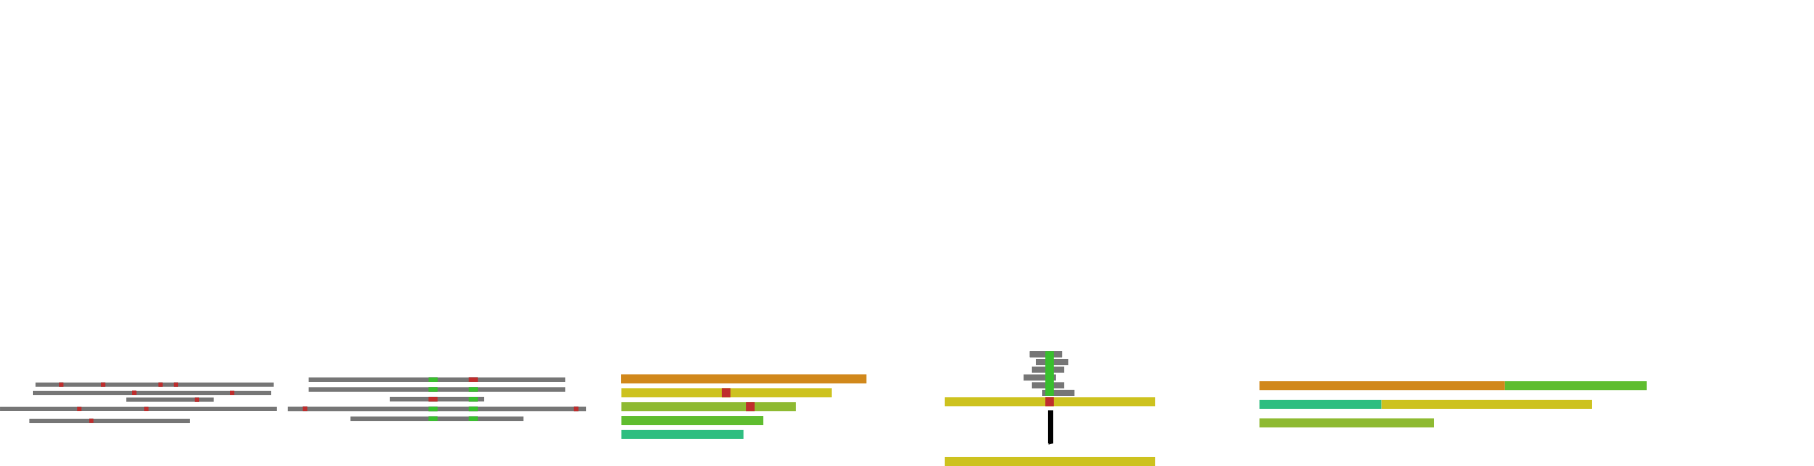
\includegraphics[width=\textwidth]{Parts/Part01/gfx/assembly_pipeline.pdf}
    \caption[Example of a third generation sequencing assembly pipeline.]{Example of a typical assembly pipeline using third generation sequencing. The error prone long reads are first corrected by pairwise comparisons. The corrected reads are assembled into contigs using their overlaps. The remaining sequencing errors in the assembly are removed by polishing with accurate short reads. Other sources of information can then be used to combine contigs into scaffolds.}
    \label{fig:01-03:assembly}
\end{figure}

\section{Phylogenetic representation}
% HGT detection requires a reference group

A common way to analyze the genome of new microorganisms is to compare it to other species. To achieve this, one needs to have other closely related genomes available. A common case where dense species genome representation is required is when attempting to detect \acrshort{HGT}.

\acrshort{HGT} detection methods often rely on discordance between gene trees and species trees. A horizontally transferred gene between two distant species would show strong sequence similarity \cite{ravenhallInferringHorizontalGene2015}. For this reason, detection of recent events requires genomes of closely related organisms as a comparison point.

\begin{figure}[htb]
    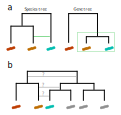
\includegraphics[width=\textwidth]{Parts/Part01/gfx/phylo_hgt.pdf}
    \caption[Phylogenetic representation of an HGT event.]{Phylogenetic representation of an HGT event. \textbf{a:} An HGT event between two species (shown with a green arrow) can be detected through discrepencies between the species (left) and gene (right) trees. \textbf{b:} In cases where genomes of closely related species are unavailable (greyed out organisms), the origin of the horizontal transfer cannot be accurately inferred (possible events shown with grey arrows).}
    \label{fig:01-03:phylo-hgt}
\end{figure}

Another frequent analysis when comparing a group of strains or species of microorganisms is to define the common set of genes they share, known as pangenome. This also allows the identification of genes specific to a particular genome, known as accessory genome. Such sets can be helpful to determine metabolic reactions associated with species or niches, however they heavily depend on the proportion of available species in the group.

Lately, several large consortia \citep{genome10kcommunityofscientistsGenome10KProposal2009,poelchauI5kWorkspaceNAL2015,DarwinTreeLife} undertook the daunting task of sequencing thousands of organisms throughout the tree of life. For the aforementioned reasons, these large collaborations are likely to greatly improve the power of comparative genomic analyses results in the future.

\section{The transition to genome graphs}

Until recently, all reference genomes were exclusively stored as linear (or circular) sequences of DNA. This linear sequence is often obtained from a mix of multiple individuals, or alleles within an individual. It is effectively a semi-arbitrary combination of multiple haplotypes collapsed into an artificial consensus sequence. A more accurate alternative is to produce a reference sequence graph instead \cite{churchExtendingReferenceAssembly2015}. Given a collection of haplotypes, individuals, or strains of a species, one can generate a graph where identical regions are collapsed, while sample-specific variants form bubbles retaining the genetic variability. As this approach is relatively recent, few algorithms have been developed to operate on sequence graphs, making their applications very limited.

The shift to genome graphs is promising for the analysis of bacterial samples, where alignment can be performed on multiple strain references at the same time. Doing this with a collection of linear genome incurs mapping bias due to ambiguous alignments between redundant regions between references \cite{liDesignConstructionReference2020}. Similarly, genome graphs also allow systematic alignment to different alleles in polyploid organisms, solving the issue of allele-specific mapping bias in linear references \cite{vandegeijnWASPAllelespecificSoftware2015}.  % Chapter 3
% Chapter X

\chapter{Thesis objectives} % Chapter title

\label{ch:01-04} % For referencing the chapter elsewhere, use \autoref{ch:name} 

Throughout this first part, we have laid out the scope of host-pathogen interactions and summarized the current state of genomics in relation to regulation and 3D genomes. Although genomics is a fast changing field, there is a need for computational tools to extract meaningful biological information from the wealth of data.

Throughout the next part, we will introduce our contributions to the field and main results. In the first chapter, we explain our methodological developments related to chromosome conformation capture technologies. In the second chapter, we will present our chromosome scale genome assembly of \textit{A. castellanii}. We then use this resource for our main findings on the genomic changes happening during infection by \textit{L. pneumophila}. Chapter 3 will focus on murine bone macrophages infection by \textit{S. enterica} and the genomic alterations it entails. Finally, in chapter 4, we will discuss additional results related to the implications of viral integrations linked to hepatocellular carcinoma in the human genome. We will end with part 3 where we discuss various aspects of genomics in infection biology, including prospects and limitations.

In this work, we develop accessible and performant methods to extract information from 3C technologies and use them to identify changes happening during infections in various organisms. We then use external data such as gene expression to assess the genes involved in those alterations and discuss how they could be associated with the infection process.
%----------------------------------------------------------------------------------------

 % Chapter 4      

%\cleardoublepage % Empty page before the start of the next part
%
%%------------------------------------------------
%
%\ctpartquote{quote}
\ctparttext{\blindtext} % Text on the Part 2 page describing the content in Part 2

\part{PART} % Second part of the thesis
% Chapter X

\chapter{CHAP} % Chapter title

\label{ch:05-01} % For referencing the chapter elsewhere, use \autoref{ch:name} 

%----------------------------------------------------------------------------------------

\section{SEC}

\blindtext % Chapter 5
%\cleardoublepage % Empty page before the start of the next part

% --------------------------
% Back matter
% --------------------------
\appendix

\ctpartquote{}
\ctparttext{}
\part{Appendices}

\chapter{Supplementary Information}
\label{sec:supdata}

 \section{Publications}
 \label{sec:appendix:publications}

    Articles published in the context of this work are included below.

    \includepdf[
        pages=-,
        addtotoc={
            1,
            subsection,
            4,
            Computer vision for pattern detection in chromosome contact maps,
            chromosight_paper
        }
    ]{Publications/chromosight_publication_supp.pdf}


%----------------------------------------------------------------------------------------
%	Glossary
%----------------------------------------------------------------------------------------
%\pagestyle{plain}
%\printglossary[type=notation]
%\clearpage

%\printglossary[type=main,style=altlist]
%\clearpage


% Bibliography
% %\renewcommand*{\bibname}{new name} % Uncomment to change the name of the bibliography
% %\setbibpreamble{} % Uncomment to include a preamble to the bibliography - some text before the reference list starts

{%
\setstretch{1.1}
\renewcommand{\bibfont}{\normalfont\small}
% \setlength{\biblabelsep}{5pt}
\setlength{\bibitemsep}{0.5\baselineskip plus 0.5\baselineskip}
\printbibliography[nottype=online,heading=bibliography]
% \printbibliography[heading=subbibliography,title={Webpages},type=online,prefixnumbers={@}]
}
\cleardoublepage

\include{FrontBackMatter/Publications} % Publications from the thesis page

\include{FrontBackMatter/Colophon}
%
% !TEX root = ../my-thesis.tex
%
%************************************************
% Declaration
%************************************************
\pdfbookmark[0]{Declaration}{Declaration}
\chapter*{Declaration}
\label{sec:declaration}
\thispagestyle{empty}

Je soussigné \thesisName~certifie que le manuscrit présenté en vue de la soutenance est le fruit d’un travail original et que toutes les sources utilisées ont été clairement indiquées.  

Je certifie, de surcroît, que je n’ai ni copié ni utilisé des idées ou des formulations tirées d’un ouvrage, article ou mémoire, en version imprimée ou électronique, sans mentionner précisément leur origine et que les citations sont expressément signalées entre guillemets (ou par une autre disposition graphique sans ambiguïté).  

Conformément à la loi, le non-respect de ces dispositions me rend passible de poursuites devant la commission disciplinaire et les tribunaux de la République française pour plagiat universitaire.


\bigskip

% \noindent\textit{\thesisUniversityCity, \thesisDate}
\noindent\textit{Fait à \thesisUniversityCity~le \thesisDate}

\smallskip

\begin{flushright}
	\begin{minipage}{5cm}
		\rule{\textwidth}{1pt}
		\centering\thesisName
	\end{minipage}
\end{flushright}

%*****************************************
%*****************************************

%\mbox{}

% **************************************************
% End of Document CONTENT
% **************************************************
\end{document}
